% !TeX program = xelatex
\documentclass[a4paper,10pt]{article}

% ============================================================================
% កញ្ចប់សម្ភារៈសិក្សាបោះពុម្ព ស-ខ្មៅ (Printable Classroom Materials - Grade 8 2.4.1 & 2.4.2 EXP412)
% ត្រូវគ្នា ១០០% នឹង LS_Plan_EXP412.tex, Teaching_Scenario_EXP412.tex និង Teaching_Guideline_EXP412.tex
% ============================================================================
\usepackage[a4paper, left=1.0cm, right=1.0cm, top=0.75cm, bottom=1.05cm, footskip=0.55cm]{geometry}
\usepackage{amsmath, amssymb}
\usepackage{unicode-math}
\usepackage{fontspec}
\usepackage{array, colortbl}
\usepackage[table]{xcolor}
\usepackage{enumitem}
\usepackage{pifont}
\usepackage{fancyhdr}
\usepackage{lastpage}
\usepackage{tikz}
\usepackage[most]{tcolorbox}
\usetikzlibrary{calc, arrows.meta, decorations.markings, decorations.pathreplacing, positioning, babel}

% LaTeX 2025 compatibility guard
\makeatletter
\let\@expl@@@mark@update@singlecol@structures@@\relax
\makeatother

% ============================================================================
% ការកំណត់ពុម្ពអក្សរផ្លូវការ (Cross-Platform Khmer + Cambria Math + Times New Roman)
% ============================================================================
\providecommand{\NGSFindFonts}{%
  \IfFileExists{C:/Windows/Fonts/cambria.ttc}{%
    \def\NGSSysPath{C:/Windows/Fonts/}%
    \def\NGSUserPath{C:/Users/KIT/AppData/Local/Microsoft/Windows/Fonts/}%
  }{%
    \IfFileExists{./fonts/KhmerOSsiemreap.ttf}{\def\NGSSysPath{./fonts/}\def\NGSUserPath{./fonts/}}{%
    \IfFileExists{../fonts/KhmerOSsiemreap.ttf}{\def\NGSSysPath{../fonts/}\def\NGSUserPath{../fonts/}}{%
    \IfFileExists{../../fonts/KhmerOSsiemreap.ttf}{\def\NGSSysPath{../../fonts/}\def\NGSUserPath{../../fonts/}}{%
    \IfFileExists{../../../fonts/KhmerOSsiemreap.ttf}{\def\NGSSysPath{../../../fonts/}\def\NGSUserPath{../../../fonts/}}{%
    \IfFileExists{../../../../fonts/KhmerOSsiemreap.ttf}{\def\NGSSysPath{../../../../fonts/}\def\NGSUserPath{../../../../fonts/}}{%
    \IfFileExists{../../../../../fonts/KhmerOSsiemreap.ttf}{\def\NGSSysPath{../../../../../fonts/}\def\NGSUserPath{../../../../../fonts/}}{%
    \IfFileExists{../../../../../../fonts/KhmerOSsiemreap.ttf}{\def\NGSSysPath{../../../../../../fonts/}\def\NGSUserPath{../../../../../../fonts/}}{%
      \def\NGSSysPath{../../../../../../../fonts/}\def\NGSUserPath{../../../../../../../fonts/}%
    }}}}}}}%
  }%
}
\NGSFindFonts

\setmathfont[
  Path={\NGSSysPath},
  FontIndex=1,
  Scale=1.02
]{cambria.ttc}

\defaultfontfeatures{Ligatures=TeX}

\setmainfont[
  Path={\NGSUserPath},
  Extension=.ttf,
  Script=Khmer,
  BoldFont={KhmerOSsiemreap},
  BoldFeatures={FakeBold=1.8},
  ItalicFont={KhmerOSsiemreap},
  ItalicFeatures={FakeSlant=0.25},
  BoldItalicFont={KhmerOSsiemreap},
  BoldItalicFeatures={FakeBold=1.8, FakeSlant=0.25}
]{KhmerOSsiemreap}

\newfontfamily\muol[
  Path={\NGSUserPath},
  Extension=.ttf,
  Script=Khmer
]{KhmerOSmuollight}

\newfontfamily\TimesEn[
  Path={\NGSSysPath},
  Extension=.ttf,
  BoldFont={timesbd},
  ItalicFont={timesi},
  BoldItalicFont={timesbi}
]{times}

\newfontfamily\CalibriFont[
  Path={\NGSSysPath},
  Extension=.ttf
]{calibri}

\newfontfamily\Tacteing[
  Path={\NGSUserPath}
]{TACTENG.TTF}

\XeTeXlinebreaklocale "km"
\XeTeXlinebreakskip = 0pt plus 1pt minus 0.1pt

% ============================================================================
% ក្ដារពណ៌ ស-ខ្មៅ សុទ្ធសម្រាប់ការបោះពុម្ព (Strict Monochrome B&W Print Palette)
% ============================================================================
\definecolor{panelgray}{gray}{0.92} % ~gray!8
\definecolor{headgray}{gray}{0.85}  % ~gray!15
\definecolor{midgray}{gray}{0.75}   % ~gray!25
\definecolor{darkline}{gray}{0.35}  % ~gray!65

\pagestyle{fancy}
\fancyhf{}
\renewcommand{\headrulewidth}{0pt}
\fancyfoot[L]{\fontsize{7.8pt}{10pt}\selectfont អនុវិទ្យាល័យព្រះក្រសាំង \en{---} គណិតវិទ្យា ថ្នាក់ទី៨ \en{|} មេរៀនទី២ (២.៤.១--២.៤.២) ស្វ័យគុណ (ស-ខ្មៅ) \en{|} ឆ្នាំមមី ២៥៧០ \en{/} ២០២៦}
\fancyfoot[R]{\fontsize{8.2pt}{10pt}\selectfont ទំព័រ \en{\thepage\ / \pageref{LastPage}}}

\setlength{\parindent}{0pt}
\setlength{\parskip}{0pt}
\setlength{\tabcolsep}{4pt}

% ============================================================================
% ម៉ាក្រូជំនួយ (Helper Macros)
% ============================================================================
\newcommand{\en}[1]{{\TimesEn #1}}
\newcommand{\enbf}[1]{{\TimesEn\bfseries #1}}
\newcommand{\unit}[1]{\,\text{\en{#1}}}
\newcommand{\cnum}[1]{\mbox{\fontsize{10pt}{12pt}\selectfont\ding{\numexpr181+#1\relax}}}
\newcommand{\cblank}{\tikz[baseline=-0.35ex]\draw[black, line width=0.8pt] (0,0) circle (0.17cm);}
\newcommand{\expbox}[1][0.40cm]{\,\tikz[baseline=-0.05ex]\draw[black, line width=0.65pt, fill=white] (0,0) rectangle (#1, 0.24cm);\,}
\newcommand{\scissors}{\ding{34}}
\newcommand{\chkbox}{\tikz[baseline=-0.15ex]\draw[black, line width=0.85pt] (0,0) rectangle (0.24cm,0.24cm);}
\newcommand{\khmflourish}{{\Tacteing\fontsize{32pt}{13pt}\selectfont\raisebox{-4pt}{3}}}

\newcommand{\pagebanner}[2]{%
  \begin{tcolorbox}[
    enhanced, sharp corners, colback=headgray, colframe=black,
    boxrule=1.1pt, boxsep=1pt, top=3pt, bottom=3pt, left=6pt, right=6pt,
    after skip=4pt
  ]
    {\muol\fontsize{9.1pt}{13.5pt}\selectfont #1}\hfill{\fontsize{8.0pt}{11.5pt}\selectfont\textbf{#2}}
  \end{tcolorbox}%
}

\newcolumntype{L}[1]{>{\raggedright\arraybackslash}p{#1}}
\newcolumntype{C}[1]{>{\centering\arraybackslash}p{#1}}

\begin{document}
\fontsize{9.0pt}{13.2pt}\selectfont

% ============================================================================
% ទំព័រទី ១៖ សម្ភារៈ E2 ខ្នាតពិត 1:1 (បន្ទះកាត់ 3x1 cm + ថាស 12 cm + ក្រឡាការ៉េ 6x6 cm + ការ៉េបង្វិល)
% ============================================================================
\pagebanner{សម្ភារៈទី ១៖ បន្ទះកាត់ \enbf{E2} ខ្នាតពិត \enbf{1:1} \enbf{\&} ផ្ទាំងពិសោធន៍ \enbf{Dual POE} ស្វ័យគុណ}{ទំព័រ ១/៦ \en{-- E2 Explore}}

% --- ប្រអប់ព្រមានខ្នាតពិត & បន្ទះផ្ទៀង 5.00 cm (x=1cm, y=1cm) ---
\noindent
\begin{minipage}[c]{11.80cm}
  \begin{tcolorbox}[
    enhanced, sharp corners, colback=panelgray, colframe=black,
    boxrule=1.0pt, boxsep=1pt, top=3pt, bottom=3pt, left=6pt, right=6pt
  ]
    \fontsize{7.8pt}{10.9pt}\selectfont
    \textbf{សេចក្ដីណែនាំបោះពុម្ពខ្នាតពិត (\en{1:1 True Scale})៖} «ពេលបោះពុម្ព សូមជ្រើស \textbf{\en{Scale: Actual Size 100\%}} \en{--} \textbf{កុំជ្រើស \en{Fit to Page}}» ដើម្បីឱ្យបន្ទះកាត់ $3.0\times 1.0\unit{cm}$, ថាស $12.0\times 1.2\unit{cm}$ និងផ្ទាំងការ៉េ $6.0\times 6.0\unit{cm}$ រក្សាខ្នាតពិត ១០០\%។\\[1.5pt]
    \textbf{ការណែនាំក្រុម (៣ នាក់)៖} ផ្ទៀងបន្ទះ \en{5.0 cm} ដោយបន្ទាត់ $\rightarrow$ ទស្សន៍ទាយ (\en{P}) $\rightarrow$ កាត់/តម្រៀបពិសោធន៍ (\en{O}) $\rightarrow$ សរសេរសន្និដ្ឋាន (\en{E})។
  \end{tcolorbox}
\end{minipage}%
\hfill
\begin{minipage}[c]{6.90cm}
  \begin{tcolorbox}[
    enhanced, sharp corners, colback=white, colframe=black,
    boxrule=1.0pt, boxsep=1pt, top=2.5pt, bottom=2.5pt, left=4pt, right=4pt
  ]
    \centering
    {\fontsize{7.6pt}{9.6pt}\selectfont\textbf{បន្ទះផ្ទៀងខ្នាតពិត \en{5.00 cm} (\en{Actual Size 100\%})}}\\[1.5pt]
    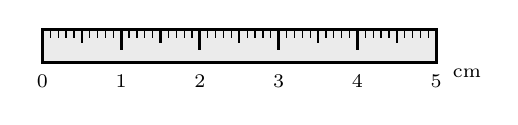
\begin{tikzpicture}[x=1cm, y=1cm, every node/.style={font=\scriptsize, text=black}]
      \draw[black, line width=1.1pt, fill=panelgray] (0,0) rectangle (5.0, 0.42);
      \foreach \m in {0,...,50}{
        \pgfmathsetmacro{\xval}{\m*0.1}
        \draw[black, line width=0.45pt] (\xval, 0.42) -- (\xval, 0.31);
      }
      \foreach \h in {0,0.5,...,5.0}{
        \draw[black, line width=0.8pt] (\h, 0.42) -- (\h, 0.24);
      }
      \foreach \c in {0,1,2,3,4,5}{
        \draw[black, line width=1.1pt] (\c, 0.42) -- (\c, 0.15);
        \node[below=1pt, font=\scriptsize] at (\c, 0.0) {\en{\c}};
      }
      \node[right=2pt, font=\scriptsize] at (5.02, -0.14) {\en{cm}};
    \end{tikzpicture}
  \end{tcolorbox}
\end{minipage}

\vspace{8pt}

% --- ស្ថានីយ៍ទី ១ (POE 1 — 4.1): បន្ទះកាត់ 4 x (3.0 cm x 1.0 cm) + ថាសគោលដៅ 12.0 cm x 1.2 cm (1:1) ---
\textbf{១. ស្ថានីយ៍ទី ១ (\en{POE 1 -- 4.1}) ៖ បន្ទះកាត់ស្វ័យគុណនៃស្វ័យគុណ $(2^3)^4$ ធៀប $2^3 \cdot 2^4$ (ខ្នាតពិត \en{x=1cm, y=1cm})}

\vspace{4pt}
\noindent
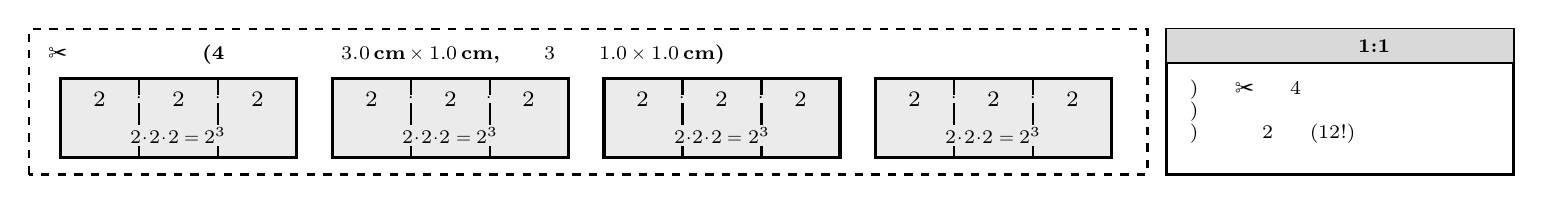
\begin{tikzpicture}[x=1cm, y=1cm, every node/.style={font=\scriptsize, text=black}]
  % Cut-out sheet with 4 exact 3.0 cm x 1.0 cm strips
  \draw[black, dashed, line width=1.0pt] (0, 0) rectangle (14.20, 1.85);
  \node[anchor=north west, font=\scriptsize] at (0.12, 1.77) {\scissors\ \textbf{សន្លឹកកាត់តាមស្នាមដាច់ (\en{4} បន្ទះ៖ បន្ទះនីមួយៗ $3.0\unit{cm} \times 1.0\unit{cm}$, បែងជា $3$ ប្លុក $1.0\times 1.0\unit{cm}$)}};
  \foreach \i/\xoff in {1/0.40, 2/3.85, 3/7.30, 4/10.75}{
    \draw[black, line width=1.2pt, fill=panelgray] (\xoff, 0.22) rectangle (\xoff+3.00, 1.22);
    \draw[black, line width=0.85pt] (\xoff+1.00, 0.22) -- (\xoff+1.00, 1.22);
    \draw[black, line width=0.85pt] (\xoff+2.00, 0.22) -- (\xoff+2.00, 1.22);
    \node[font=\footnotesize] at (\xoff+0.50, 0.96) {$2$};
    \node[font=\footnotesize] at (\xoff+1.50, 0.96) {$2$};
    \node[font=\footnotesize] at (\xoff+2.50, 0.96) {$2$};
    \node[font=\scriptsize, fill=panelgray, inner sep=0.4pt] at (\xoff+1.00, 0.96) {$\cdot$};
    \node[font=\scriptsize, fill=panelgray, inner sep=0.4pt] at (\xoff+2.00, 0.96) {$\cdot$};
    \node[font=\scriptsize, fill=panelgray, inner sep=0.8pt] at (\xoff+1.50, 0.50) {$2\!\cdot\! 2\!\cdot\! 2 = 2^3$};
  }

  % Instruction side box (14.45 .. 18.85)
  \draw[black, line width=1.0pt, fill=white] (14.45, 0.0) rectangle (18.85, 1.85);
  \fill[headgray] (14.45, 1.42) rectangle (18.85, 1.85);
  \draw[black, line width=0.8pt] (14.45, 1.42) -- (18.85, 1.42);
  \node[font=\scriptsize] at (16.65, 1.63) {\textbf{វិធីពិសោធន៍ \en{1:1}}};
  \node[anchor=north west, align=left, font=\scriptsize] at (14.55, 1.33) {១) កាត់ \scissors\ ទាំង $4$ បន្ទះ\\ ២) ដាក់តម្រៀបចូលថាស\\ ៣) រាប់កត្តា $2$ សរុប ($12$!)};
\end{tikzpicture}

\vspace{5pt}
\noindent
\begin{minipage}[c]{12.60cm}
  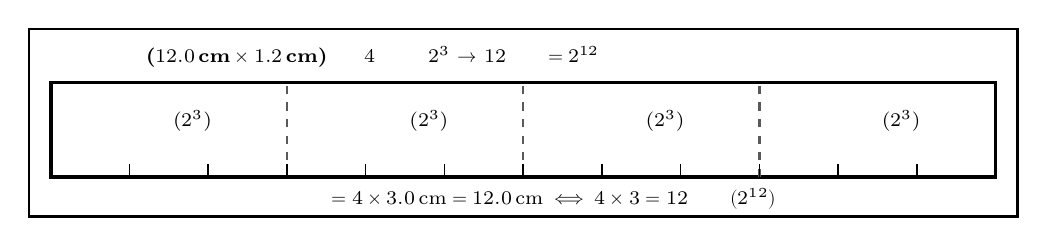
\begin{tikzpicture}[x=1cm, y=1cm, every node/.style={font=\scriptsize, text=black}]
    % Exact 12.0 cm x 1.2 cm Target Tray
    \draw[black, line width=1.0pt] (0, 0) rectangle (12.55, 2.38);
    \node[anchor=north west, font=\scriptsize] at (0.15, 2.29) {\textbf{ថាសគោលដៅខ្នាតពិត ($12.0\unit{cm}\times 1.2\unit{cm}$)}៖ បើក $4$ ក្រុមនៃ $2^3$ $\to$ $12$ កត្តា $= 2^{12}$};
    \draw[black, line width=1.3pt, fill=white] (0.275, 0.50) rectangle (12.275, 1.70);
    \foreach \g in {3, 6, 9}{
      \draw[darkline, dashed, line width=0.85pt] (0.275+\g, 0.50) -- (0.275+\g, 1.70);
    }
    \foreach \k in {1,2,...,11}{
      \draw[black, line width=0.55pt] (0.275+\k, 0.50) -- (0.275+\k, 0.66);
    }
    \foreach \g/\lbl in {1.5/ក្រុម ១ ($2^3$), 4.5/ក្រុម ២ ($2^3$), 7.5/ក្រុម ៣ ($2^3$), 10.5/ក្រុម ៤ ($2^3$)}{
      \node[font=\scriptsize] at (0.275+\g, 1.22) {\lbl};
    }
    \node[font=\scriptsize] at (6.275, 0.22) {ប្រវែងសរុប $= 4 \times 3.0\unit{cm} = 12.0\unit{cm} \iff 4 \times 3 = 12\text{ កត្តា } (2^{12})$};
  \end{tikzpicture}
\end{minipage}%
\hfill
\begin{minipage}[c]{6.32cm}
  \begin{tcolorbox}[
    enhanced, sharp corners, colback=panelgray, colframe=black,
    boxrule=0.95pt, boxsep=1pt, top=4.5pt, bottom=4.5pt, left=5pt, right=5pt
  ]
    \raggedright\fontsize{7.3pt}{10.8pt}\selectfont
    \textbf{\en{P} -- ទស្សន៍ទាយ (\en{Predict})៖}\\[2pt]
    $(2^3)^4 =$ \chkbox~$2^7$ (សុខ) \;\; \chkbox~$2^{12}$ (\mbox{បូណា})\\[4pt]
    \textbf{\en{O} -- សង្កេត (\en{Observe})៖}\\[2pt]
    $\bullet$ $4$ បន្ទះក្នុងថាស $= 2^{\expbox}$ ($12$ កត្តា) \chkbox\\[2.5pt]
    $\bullet$ ខុសពី $2^3\cdot 2^4 = 2^{\expbox}$ (មានតែ $7$ កត្តា!) \chkbox
  \end{tcolorbox}
\end{minipage}

\vspace{11pt}

% --- ស្ថានីយ៍ទី ២ (POE 2 — 4.2): ក្រឡាការ៉េ 6.0 cm x 6.0 cm (1:1) + ការ៉េបង្វិល ~25° (2+3)^2 != 2^2+3^2 ---
\textbf{២. ស្ថានីយ៍ទី ២ (\en{POE 2 -- 4.2}) ៖ ក្រឡាការ៉េ $(3b)^2 = 9b^2$ ($6.0\times 6.0\unit{cm}$) និងអន្ទាក់លីនេអ៊ែរ $(2+3)^2 \neq 2^2+3^2$ (ខ្នាតពិត \en{x=1cm, y=1cm})}

\vspace{4pt}
\noindent
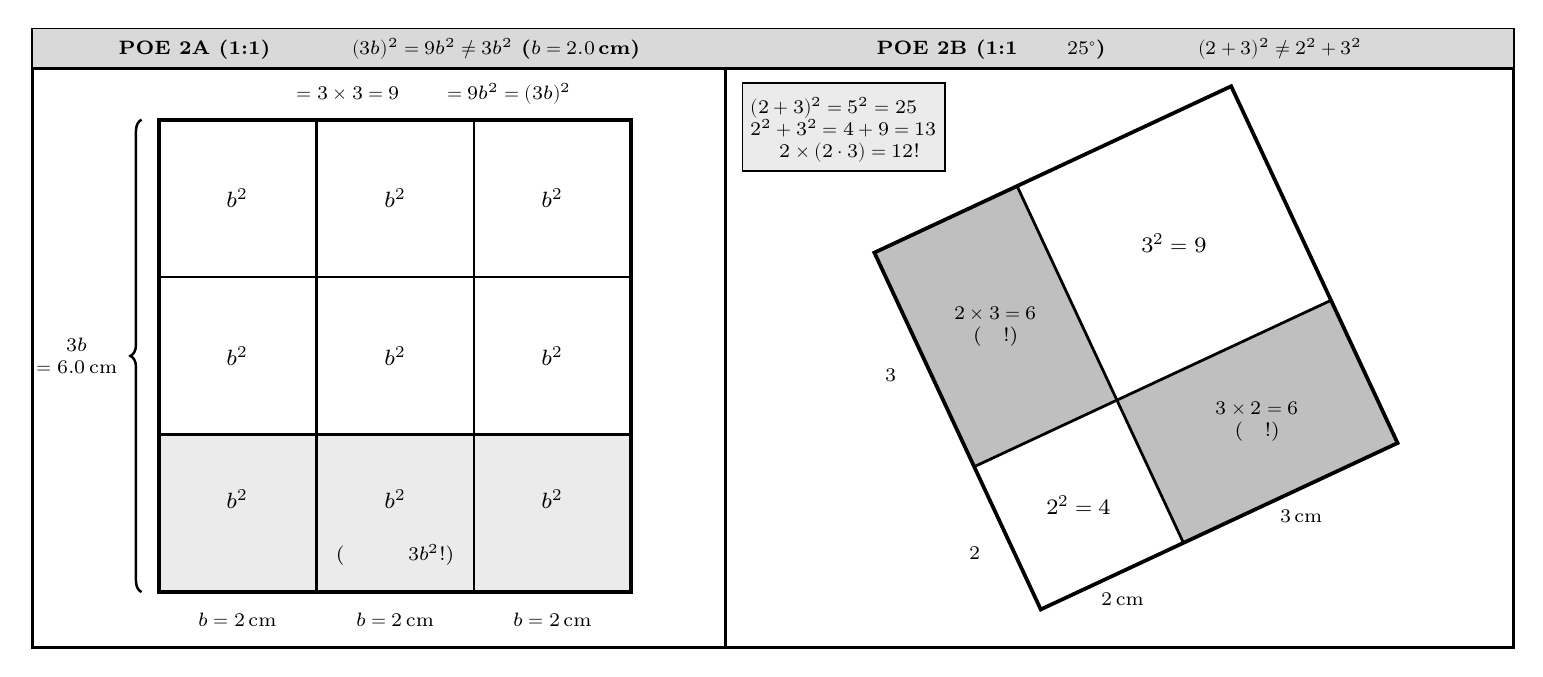
\begin{tikzpicture}[x=1cm, y=1cm, every node/.style={font=\scriptsize, text=black}]
  % Outer frame
  \draw[black, line width=1.05pt] (0, 0) rectangle (18.80, 7.85);
  \draw[black, line width=0.95pt] (8.80, 0) -- (8.80, 7.85);

  % === Left Panel: 6.0 cm x 6.0 cm (3b)^2 = 9b^2 Grid Mat ===
  \fill[headgray] (0, 7.35) rectangle (8.80, 7.85);
  \draw[black, line width=0.85pt] (0, 7.35) -- (8.80, 7.35);
  \node[font=\scriptsize] at (4.40, 7.60) {\textbf{\en{POE 2A (1:1)}៖ ផ្ទាំងការ៉េ $(3b)^2 = 9b^2 \neq 3b^2$ ($b = 2.0\unit{cm}$)}};

  % Highlight bottom row (3 tiles = 3b^2) in light gray to contrast with 9 tiles = 9b^2
  \fill[panelgray] (1.60, 0.70) rectangle (7.60, 2.70);
  % 3x3 grid of 2.0 cm x 2.0 cm tiles from (1.60, 0.70) to (7.60, 6.70)
  \draw[black, line width=1.35pt] (1.60, 0.70) rectangle (7.60, 6.70);
  \draw[black, line width=0.9pt] (3.60, 0.70) -- (3.60, 6.70);
  \draw[black, line width=0.9pt] (5.60, 0.70) -- (5.60, 6.70);
  \draw[black, line width=0.9pt] (1.60, 2.70) -- (7.60, 2.70);
  \draw[black, line width=0.9pt] (1.60, 4.70) -- (7.60, 4.70);

  \foreach \xval in {2.60, 4.60, 6.60}{
    \node[font=\footnotesize] at (\xval, 1.88) {$b^2$};
    \node[font=\footnotesize] at (\xval, 3.70) {$b^2$};
    \node[font=\footnotesize] at (\xval, 5.70) {$b^2$};
  }
  \node[font=\scriptsize] at (4.60, 1.18) {(សុខ៖ គិតតែ $3b^2$!)};
  \node[font=\scriptsize, fill=white, inner sep=1pt] at (4.60, 7.03) {ផ្ទៃក្រឡាសរុប $= 3\times 3 = 9$ ផ្ទាំង $= 9b^2 = (3b)^2$};

  % Left side vertical brace (3b = 6.0 cm)
  \draw[decorate, decoration={brace, amplitude=4pt}, line width=0.9pt] (1.38, 0.70) -- (1.38, 6.70)
    node[midway, left=5pt, align=center, font=\scriptsize] {$3b$\\$= 6.0\unit{cm}$};
  % Bottom width ticks (2.0 cm each)
  \node[font=\scriptsize] at (2.60, 0.35) {$b=2\unit{cm}$};
  \node[font=\scriptsize] at (4.60, 0.35) {$b=2\unit{cm}$};
  \node[font=\scriptsize] at (6.60, 0.35) {$b=2\unit{cm}$};

  % === Right Panel: Rotated (~25 deg) True 1:1 5x5 Counter-Example (2+3)^2 != 2^2 + 3^2 ===
  \fill[headgray] (8.80, 7.35) rectangle (18.80, 7.85);
  \draw[black, line width=0.85pt] (8.80, 7.35) -- (18.80, 7.35);
  \node[font=\scriptsize] at (13.80, 7.60) {\textbf{\en{POE 2B (1:1} បង្វិល $25^\circ$)៖ ឧទាហរណ៍ជំទាស់ $(2+3)^2 \neq 2^2+3^2$}};

  % Rotate 25 deg around origin (12.80, 0.48)
  \begin{scope}[shift={(12.80, 0.48)}, rotate=25]
    % Two lost cross-rectangles 2x3 = 6 shaded midgray
    \fill[midgray] (0, 2) rectangle (2, 5);
    \fill[midgray] (2, 0) rectangle (5, 2);
    % White squares 2^2=4 and 3^2=9
    \fill[white] (0, 0) rectangle (2, 2);
    \fill[white] (2, 2) rectangle (5, 5);
    % Thick outer boundary & inner partition lines
    \draw[black, line width=1.35pt] (0, 0) rectangle (5, 5);
    \draw[black, line width=1.0pt] (2, 0) -- (2, 5);
    \draw[black, line width=1.0pt] (0, 2) -- (5, 2);
    % Labels inside the 4 sub-regions
    \node[font=\footnotesize] at (1.0, 1.0) {$2^2=4$};
    \node[font=\footnotesize] at (3.5, 3.5) {$3^2=9$};
    \node[align=center, font=\scriptsize] at (1.0, 3.5) {$2\times 3 = 6$\\(បាត់!)};
    \node[align=center, font=\scriptsize] at (3.5, 1.0) {$3\times 2 = 6$\\(បាត់!)};
    % Side segment labels cleanly outside
    \node[font=\scriptsize] at (1.0, -0.32) {$2\unit{cm}$};
    \node[font=\scriptsize] at (3.5, -0.32) {$3\unit{cm}$};
    \node[font=\scriptsize] at (-0.46, 1.0) {$2$};
    \node[font=\scriptsize] at (-0.46, 3.5) {$3$};
  \end{scope}

  % Summary callout at top-left of Right Panel
  \node[anchor=north west, draw=black, line width=0.7pt, fill=panelgray, inner sep=3pt, align=left, font=\scriptsize] at (9.00, 7.18)
    {\textbf{ផ្ទៀងផ្ទាត់៖}\\$(2+3)^2 = 5^2 = 25$\\$2^2+3^2 = 4+9 = 13$\\បាត់ $2\times(2\cdot 3) = 12$!};
\end{tikzpicture}

\vspace{11pt}

% --- តារាងកំណត់ត្រា POE 2 & សន្និដ្ឋាន E2 (Predict - Observe - Explain) ---
\begin{tcolorbox}[
  enhanced, sharp corners, colback=white, colframe=black,
  boxrule=1.0pt, boxsep=1pt, top=9pt, bottom=9pt, left=7pt, right=7pt
]
  \raggedright\fontsize{8.2pt}{12.0pt}\selectfont
  \textbf{\en{P} -- ទស្សន៍ទាយមុនរាប់ (\en{Predict})៖}\quad
  \textbf{១)} ការ៉េជ្រុង $3b$ ត្រូវការប៉ុន្មានផ្ទាំង $b^2$? \chkbox~$3b^2$ (សុខ) \quad \chkbox~$9b^2$ (\mbox{បូណា}) \qquad
  \textbf{២)} តើ $(2+3)^2 = 2^2+3^2$ ឬទេ? \chkbox~ស្មើ \quad \chkbox~មិនស្មើ\\[7pt]

  \textbf{\en{O} -- តារាងសង្កេតរង្វាស់ខ្នាតពិត \en{1:1} (\en{Observe})៖}\\[4pt]
  \renewcommand{\arraystretch}{1.48}
  \begin{tabular}{|L{4.00cm}|L{9.10cm}|L{4.20cm}|}
    \hline
    \cellcolor{headgray}\textbf{ផ្ទាំងពិសោធន៍ \en{POE 2}} & \cellcolor{headgray}\textbf{រង្វាស់ខ្នាតពិត \en{1:1} និងការផ្គុំផលគុណ (ទំ.១៧)} & \cellcolor{headgray}\textbf{លទ្ធផលពិសោធន៍} \\ \hline
    \textbf{\en{POE 2A}}៖ ក្រឡា $6.0\times 6.0\unit{cm}$ & $1$ ផ្ទាំង $= 2\times 2 = 4\unit{cm}^2$ ($b^2$) \en{|} រាប់បាន $\underline{\hspace{0.55cm}}$ ផ្ទាំង ($3\times 3$) & $(3b)^2 = \underline{\hspace{0.55cm}}b^2 \neq 3b^2$ \\ \hline
    \textbf{\en{POE 2B}}៖ ការ៉េ $(2+3)^2$ & $2^2+3^2 = 13$ \en{|} ចតុកោណកែងប្រផេះដែលបាត់ $= 2\times(\underline{\hspace{0.5cm}}) = \underline{\hspace{0.5cm}}$ & $(2+3)^2 = 25 \neq 13$! \\ \hline
    \textbf{ទំ.១៧ (ក--គ)}៖ ផ្គុំកត្តា & $2^3\cdot 5^3 = (2\times 5)^{\expbox} = \underline{\hspace{0.9cm}}$ \en{|} $2^2\cdot 5^2\cdot 7^2 = (2\times 5\times 7)^{\expbox}$ & ទូទៅ៖ $a^n b^n = (ab)^n$ \\ \hline
  \end{tabular}\\[8pt]

  \textbf{\en{E} -- ពន្យល់សន្និដ្ឋាន (\en{Explain})៖} (១) ស្វ័យគុណនៃស្វ័យគុណ $(a^m)^n = a^{\expbox[0.60cm]}$ (គុណនិទស្សន្ត មិនមែនបូក!)។ (២) ស្វ័យគុណចែកចាយលើ\textbf{ផលគុណ} $(ab)^n = a^n b^n$ ប៉ុន្តែ\textbf{ហាម}ចែកចាយលើផលបូក $(a+b)^n \neq a^n+b^n$!\\[7pt]
  \textbf{សង្ខេបក្រុមផ្ទាល់ដៃ៖} ហេតុអ្វី $(3b)^2 = 9b^2$ និង $(2+3)^2 \neq 2^2+3^2$? $\underline{\hspace{11.4cm}}$\\[6pt]
  \hspace*{1.4cm} $\underline{\hspace{16.4cm}}$
\end{tcolorbox}

\clearpage

% ============================================================================
% ទំព័រទី ២៖ E4 កាតស៊ើបអង្កេតសញ្ញាគន្លឹះ ៣ ជំហាន (គំរូ ៤.១ & ៤.២ ទំ.១៧–១៨ ដើម) + EIA
% ============================================================================
\pagebanner{សម្ភារៈទី ២៖ កាត \enbf{E4} «កាតស៊ើបអង្កេតសញ្ញាគន្លឹះ ៣ ជំហាន» \enbf{(}លំហាត់គំរូ ទំ.១៧\enbf{--}១៨ ដើម\enbf{)}}{ទំព័រ ២/៦ \en{-- E4 Elaborate}}

\vspace{6pt}
% --- កាតទី ១៖ គំរូ 4.1 ក & ខ (ទំ.១៧) ---
\begin{tcolorbox}[
  enhanced, sharp corners, colback=white, colframe=white,
  borderline={1.0pt}{0pt}{black, dashed},
  boxsep=1pt, top=8pt, bottom=8pt, left=6pt, right=6pt
]
  \begin{tcolorbox}[
    enhanced, sharp corners, colback=headgray, colframe=black,
    boxrule=0.85pt, boxsep=1pt, top=4pt, bottom=4pt, left=5pt, right=5pt, after skip=7pt
  ]
    \fontsize{8.5pt}{11.8pt}\selectfont
    \textbf{\scissors\ កាតស៊ើបអង្កេតទី ១ \en{--} គំរូ \en{4.1} (ទំ.១៧)៖} \textbf{ក.} $(10^2)^3$ \qquad \textbf{ខ.} $(a^{-2})^k \cdot (a^k)^5$ ($a \neq 0$) \hfill ក្រុម៖ $\underline{\hspace{2.6cm}}$
  \end{tcolorbox}

  \renewcommand{\arraystretch}{1.35}
  {\centering\setlength{\tabcolsep}{4.5pt}%
  \begin{tabular}{|L{5.65cm}|L{5.65cm}|L{6.05cm}|}
    \hline
    \cellcolor{panelgray}\centering\arraybackslash\fontsize{8.0pt}{11.0pt}\selectfont\textbf{ជំហាន ១៖ ព័ទ្ធក្រុម \& អូសដាន \en{[tracing]}} &
    \cellcolor{panelgray}\centering\arraybackslash\fontsize{8.0pt}{11.0pt}\selectfont\textbf{ជំហាន ២៖ ភ្ជាប់ហេតុផល \cnum{1}--\cnum{5}} &
    \cellcolor{panelgray}\centering\arraybackslash\fontsize{8.0pt}{11.0pt}\selectfont\textbf{ជំហាន ៣៖ គណនា \& ផ្ទៀងលក្ខខណ្ឌ} \\ \hline

    \fontsize{8.1pt}{12.0pt}\selectfont
    \textbf{ក.} អូសដានម្រាមដៃឆ្លងវង់ក្រចក៖\newline
    $\big[\,10^2\,\big]^3 \implies$ និទស្សន្ត $2$ ជួប $3$!\par\vspace{7pt}
    \textbf{ខ.} ព័ទ្ធពីរក្រុមដាច់ដោយឡែក៖\newline
    $\big[\,a^{-2}\,\big]^k \cdot \big[\,a^k\,\big]^5$ ($a \neq 0$)
    &
    \fontsize{8.1pt}{12.0pt}\selectfont
    \textbf{ក.} ប្រើហេតុផលលេខ \chkbox~\cnum{1} \chkbox~\cnum{4}៖\newline
    $(a^m)^n = a^{m\cdot n}$ (គុណនិទស្សន្ត)\par\vspace{7pt}
    \textbf{ខ.} ជំហានដោះស្រាយ៖\newline
    ដំបូងគុណនិទស្សន្ត (\cblank) រួចគុណគោល $a$ ដូចគ្នា (\cblank)។
    &
    \fontsize{8.1pt}{12.0pt}\selectfont
    \textbf{ក.} $(10^2)^3 = 10^{2\times 3} = 10^{\expbox} = \underline{\hspace{1.45cm}}$ \chkbox\par\vspace{5pt}
    \textbf{ខ.} $(a^{-2})^k \cdot (a^k)^5 = a^{\expbox[0.52cm]} \cdot a^{\expbox[0.52cm]}$\newline
    \hspace*{1.2em} $= a^{-2k + 5k} = a^{\expbox[0.52cm]}$ ($a \neq 0$) \chkbox
    \\ \hline
  \end{tabular}\par}
\end{tcolorbox}

\vspace{12pt}

% --- កាតទី ២៖ គំរូ 4.2 ក & ខ (ទំ.១៨ ដើម) + រូប B&W Scope-Bracketing ---
\begin{tcolorbox}[
  enhanced, sharp corners, colback=white, colframe=white,
  borderline={1.0pt}{0pt}{black, dashed},
  boxsep=1pt, top=8pt, bottom=8pt, left=6pt, right=6pt
]
  \begin{tcolorbox}[
    enhanced, sharp corners, colback=headgray, colframe=black,
    boxrule=0.85pt, boxsep=1pt, top=4pt, bottom=4pt, left=5pt, right=5pt, after skip=7pt
  ]
    \fontsize{8.5pt}{11.8pt}\selectfont
    \textbf{\scissors\ កាតស៊ើបអង្កេតទី ២ \en{--} គំរូ \en{4.2} (ទំ.១៨ ដើម)៖} \textbf{ក.} $(3xy^2)^3$ \qquad \textbf{ខ.} $(b^3)(b^{2k-1})^3$ ($b \neq 0$) \hfill ក្រុម៖ $\underline{\hspace{2.6cm}}$
  \end{tcolorbox}

  \renewcommand{\arraystretch}{1.35}
  {\centering\setlength{\tabcolsep}{4.5pt}%
  \begin{tabular}{|L{5.65cm}|L{5.65cm}|L{6.05cm}|}
    \hline
    \cellcolor{panelgray}\centering\arraybackslash\fontsize{8.0pt}{11.0pt}\selectfont\textbf{ជំហាន ១៖ ព័ទ្ធក្រុម \& អូសដាន \en{[tracing]}} &
    \cellcolor{panelgray}\centering\arraybackslash\fontsize{8.0pt}{11.0pt}\selectfont\textbf{ជំហាន ២៖ ភ្ជាប់ហេតុផល \cnum{1}--\cnum{5}} &
    \cellcolor{panelgray}\centering\arraybackslash\fontsize{8.0pt}{11.0pt}\selectfont\textbf{ជំហាន ៣៖ គណនា \& ផ្ទៀងលក្ខខណ្ឌ} \\ \hline

    \fontsize{8.1pt}{12.0pt}\selectfont
    \textbf{ក.} បង្ហាញមេគុណ និងនិទស្សន្តលាក់ $1$៖\newline
    $\big(\,[3] \cdot [x^1] \cdot [y^2]\,\big)^3$ (មាន $3$ កត្តា!)\par\vspace{7pt}
    \textbf{ខ.} ព័ទ្ធកន្សោម $2k-1$ ជាប្លុកតែមួយ៖\newline
    $(b^3) \cdot \big[\,b^{(2k-1)}\,\big]^3$ ($b \neq 0$)
    &
    \fontsize{8.1pt}{12.0pt}\selectfont
    \textbf{ក.} ចែក $3$ ឱ្យទាំង $3$ កត្តា (\cblank) រួចគុណនិទស្សន្តលើ $(y^2)^3$ (\cblank)។\par\vspace{7pt}
    \textbf{ខ.} គុណ $3$ ចូល\textbf{គ្រប់តួ}ក្នុង $(2k-1)$ (\cnum{1}) រួចបូកនិទស្សន្តគោល $b$ (\cnum{4})។
    &
    \fontsize{8.1pt}{12.0pt}\selectfont
    \textbf{ក.} $(3xy^2)^3 = 3^{\expbox}\cdot x^{\expbox}\cdot (y^2)^{\expbox}$\newline
    \hspace*{1.2em} $= 3^{\expbox}\cdot x^{\expbox}\cdot y^{\expbox} = \underline{\hspace{1.45cm}}$ \chkbox\par\vspace{5pt}
    \textbf{ខ.} $(b^3)(b^{2k-1})^3 = b^3 \cdot b^{3(2k-1)}$\newline
    \hspace*{1.2em} $= b^{3 + \expbox[0.80cm]} = b^{\expbox[0.52cm]}$ ($b \neq 0$) \chkbox
    \\ \hline
  \end{tabular}\par}

  \vspace{10pt}
  % --- ដ្យាក្រាម ស-ខ្មៅ ប្រៀបធៀបដែនវង់ក្រចក (B&W Scope-Bracketing Diagram) ---
  \noindent
  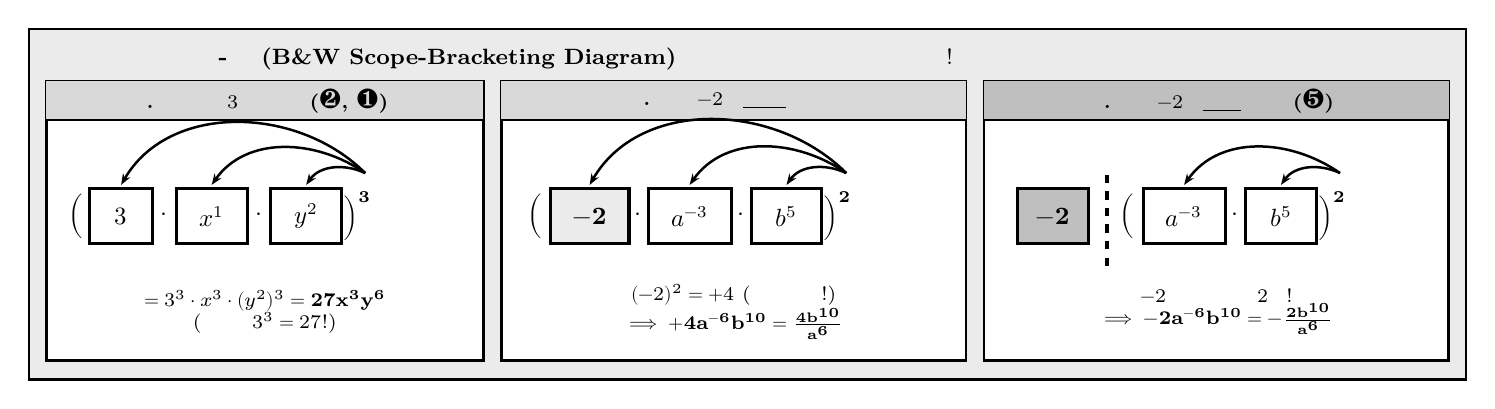
\begin{tikzpicture}[x=1cm, y=1cm, every node/.style={font=\footnotesize, text=black}]
    \draw[black, line width=0.95pt, fill=panelgray] (0, 0) rectangle (18.25, 4.45);
    \node[anchor=north west, font=\footnotesize] at (0.20, 4.33) {\textbf{រូបវិភាគវិសាលភាពវង់ក្រចក ស-ខ្មៅ (\en{B\&W Scope-Bracketing Diagram})៖} ពិនិត្យកត្តានៅ\textbf{ខាងក្នុង} និង\textbf{ខាងក្រៅ}វង់ក្រចក!};

    % Left sub-box: [3]*[x^1]*[y^2]
    \begin{scope}[shift={(0.22, 0.24)}]
      \draw[black, line width=0.95pt, fill=white] (0, 0) rectangle (5.55, 3.55);
      \fill[headgray] (0, 3.05) rectangle (5.55, 3.55);
      \draw[black, line width=0.8pt] (0, 3.05) -- (5.55, 3.05);
      \node[font=\scriptsize] at (2.775, 3.30) {\textbf{១. ព័ទ្ធកត្តា $3$ ដាច់ដោយឡែក \en{(\cnum{2}, \cnum{1})}}};

      \draw[black, line width=1.1pt] (0.55, 1.48) rectangle (1.35, 2.18);
      \draw[black, line width=1.1pt] (1.65, 1.48) rectangle (2.55, 2.18);
      \draw[black, line width=1.1pt] (2.85, 1.48) rectangle (3.75, 2.18);
      \node[font=\small] at (0.95, 1.83) {$3$};
      \node[font=\small] at (1.50, 1.83) {$\cdot$};
      \node[font=\small] at (2.10, 1.83) {$x^1$};
      \node[font=\small] at (2.70, 1.83) {$\cdot$};
      \node[font=\small] at (3.30, 1.83) {$y^2$};
      \node[font=\small] at (0.38, 1.83) {$\Big($};
      \node[font=\small] at (3.95, 1.83) {$\Big)^{\mathbf{3}}$};

      \draw[black, line width=0.9pt, -{Stealth[length=1.4mm]}] (4.05, 2.38) to[out=135, in=60] (0.95, 2.23);
      \draw[black, line width=0.9pt, -{Stealth[length=1.4mm]}] (4.05, 2.38) to[out=145, in=55] (2.10, 2.23);
      \draw[black, line width=0.9pt, -{Stealth[length=1.4mm]}] (4.05, 2.38) to[out=155, in=55] (3.30, 2.23);

      \node[align=center, font=\scriptsize] at (2.775, 0.62) {$= 3^3 \cdot x^3 \cdot (y^2)^3 = \mathbf{27x^3y^6}$\\(ហាមភ្លេច $3^3 = 27$!)};
    \end{scope}

    % Middle sub-box: (-2 a^{-3} b^5)^2 (INSIDE brackets)
    \begin{scope}[shift={(6.00, 0.24)}]
      \draw[black, line width=0.95pt, fill=white] (0, 0) rectangle (5.90, 3.55);
      \fill[headgray] (0, 3.05) rectangle (5.90, 3.55);
      \draw[black, line width=0.8pt] (0, 3.05) -- (5.90, 3.05);
      \node[font=\scriptsize] at (2.95, 3.30) {\textbf{២. មេគុណ $-2$ នៅ\underline{ខាងក្នុង}វង់ក្រចក}};

      \draw[black, line width=1.1pt, fill=panelgray] (0.62, 1.48) rectangle (1.62, 2.18);
      \draw[black, line width=1.1pt] (1.87, 1.48) rectangle (2.92, 2.18);
      \draw[black, line width=1.1pt] (3.17, 1.48) rectangle (4.07, 2.18);
      \node[font=\small] at (1.12, 1.83) {$\mathbf{-2}$};
      \node[font=\small] at (1.74, 1.83) {$\cdot$};
      \node[font=\small] at (2.39, 1.83) {$a^{-3}$};
      \node[font=\small] at (3.04, 1.83) {$\cdot$};
      \node[font=\small] at (3.62, 1.83) {$b^5$};
      \node[font=\small] at (0.42, 1.83) {$\Big($};
      \node[font=\small] at (4.27, 1.83) {$\Big)^{\mathbf{2}}$};

      \draw[black, line width=0.9pt, -{Stealth[length=1.4mm]}] (4.38, 2.38) to[out=135, in=60] (1.12, 2.23);
      \draw[black, line width=0.9pt, -{Stealth[length=1.4mm]}] (4.38, 2.38) to[out=145, in=55] (2.39, 2.23);
      \draw[black, line width=0.9pt, -{Stealth[length=1.4mm]}] (4.38, 2.38) to[out=155, in=55] (3.62, 2.23);

      \node[align=center, font=\scriptsize] at (2.95, 0.62) {$(-2)^2 = +4$ (ត្រូវលើកការ៉េ!)\\$\implies \mathbf{+4a^{-6}b^{10} = \frac{4b^{10}}{a^6}}$};
    \end{scope}

    % Right sub-box: -2(a^{-3} b^5)^2 (OUTSIDE brackets)
    \begin{scope}[shift={(12.13, 0.24)}]
      \draw[black, line width=0.95pt, fill=white] (0, 0) rectangle (5.90, 3.55);
      \fill[midgray] (0, 3.05) rectangle (5.90, 3.55);
      \draw[black, line width=0.8pt] (0, 3.05) -- (5.90, 3.05);
      \node[font=\scriptsize] at (2.95, 3.30) {\textbf{៣. មេគុណ $-2$ នៅ\underline{ខាងក្រៅ}វង់ក្រចក \en{(\cnum{5})}}};

      \draw[black, line width=1.1pt, fill=midgray] (0.42, 1.48) rectangle (1.32, 2.18);
      \node[font=\small] at (0.87, 1.83) {$\mathbf{-2}$};
      \draw[black, dashed, line width=1.3pt] (1.56, 1.20) -- (1.56, 2.40);
      \node[font=\scriptsize] at (1.56, 2.66) {ជញ្ជាំង};

      \draw[black, line width=1.1pt] (2.02, 1.48) rectangle (3.07, 2.18);
      \draw[black, line width=1.1pt] (3.32, 1.48) rectangle (4.22, 2.18);
      \node[font=\small] at (2.54, 1.83) {$a^{-3}$};
      \node[font=\small] at (3.19, 1.83) {$\cdot$};
      \node[font=\small] at (3.77, 1.83) {$b^5$};
      \node[font=\small] at (1.82, 1.83) {$\Big($};
      \node[font=\small] at (4.42, 1.83) {$\Big)^{\mathbf{2}}$};

      \draw[black, line width=0.9pt, -{Stealth[length=1.4mm]}] (4.52, 2.38) to[out=145, in=55] (2.54, 2.23);
      \draw[black, line width=0.9pt, -{Stealth[length=1.4mm]}] (4.52, 2.38) to[out=155, in=55] (3.77, 2.23);

      \node[align=center, font=\scriptsize] at (2.95, 0.62) {$-2$ \textbf{មិន}លើកស្វ័យគុណ $2$ ទេ!\\$\implies \mathbf{-2a^{-6}b^{10} = -\frac{2b^{10}}{a^6}}$};
    \end{scope}
  \end{tikzpicture}
\end{tcolorbox}

\vspace{13pt}

% --- ប្រអប់ EIA Looking-Back Prompts & Warrant Bank Mini-Bar ---
\begin{tcolorbox}[
  enhanced, sharp corners, colback=panelgray, colframe=black,
  boxrule=1.0pt, boxsep=1pt, top=8pt, bottom=9pt, left=7pt, right=7pt,
  title={\textbf{ពិនិត្យត្រឡប់ក្រោយ (\en{EIA Looking-Back Prompts} -- ចាប់កំហុស)}},
  colbacktitle=headgray, coltitle=black, fonttitle=\fontsize{8.8pt}{12.0pt}\selectfont
]
  \raggedright\fontsize{8.4pt}{12.8pt}\selectfont
  \textbf{១)} ហេតុអ្វី $(3xy^2)^3 = 3x^3y^6$ ឬ $(3xy^2)^3 = 9x^3y^5$ \textbf{ខុស}? ចូរពន្យល់ដោយប្រើ \cnum{2} និង \cnum{1}៖\\[6pt]
  \hspace*{1.2em} $\triangleright$ $\underline{\hspace{16.2cm}}$\\[9pt]
  \hspace*{1.2em} \hspace*{0.85em} $\underline{\hspace{16.2cm}}$\\[9pt]
  \hspace*{1.2em} \hspace*{0.85em} $\underline{\hspace{16.2cm}}$\\[11pt]
  \textbf{២)} ហេតុអ្វី $b^{3(2k-1)} \neq b^{6k-1}$? ចូរពន្យល់ពីការគុណបំបែកវង់ក្រចកលើនិទស្សន្ត៖\\[6pt]
  \hspace*{1.2em} $\triangleright$ $\underline{\hspace{16.2cm}}$\\[9pt]
  \hspace*{1.2em} \hspace*{0.85em} $\underline{\hspace{16.2cm}}$\\[9pt]
  \hspace*{1.2em} \hspace*{0.85em} $\underline{\hspace{16.2cm}}$
\end{tcolorbox}

\vspace{11pt}
\begin{tcolorbox}[
  enhanced, sharp corners, colback=white, colframe=black,
  boxrule=0.85pt, boxsep=1pt, top=5pt, bottom=5pt, left=6pt, right=6pt
]
  \centering\fontsize{7.8pt}{11.0pt}\selectfont
  \textbf{ធនាគារហេតុផល \cnum{1}--\cnum{5}៖}
  \cnum{1} $(a^m)^n=a^{mn}$ \en{|}
  \cnum{2} $(ab)^n=a^nb^n$ \en{|}
  \cnum{3} $a^nb^n=(ab)^n$ \en{|}
  \cnum{4} $a^ma^n=a^{m+n},\; a=a^1$ \en{|}
  \cnum{5} $a^{-n}=\frac{1}{a^n},\; a^0=1\; (a\neq 0),\; -c(ab)^n\neq(-cab)^n$
\end{tcolorbox}

\clearpage

% ============================================================================
% ទំព័រទី ៣៖ E5 បេសកកម្មសហការ ៣ តួនាទី (Proof Relay — ប្រតិបត្តិ ៤.១ ទំ.១៧ & ៤.២ ទំ.១៨ ដើម)
% ============================================================================
\pagebanner{សម្ភារៈទី ៣៖ សន្លឹក \enbf{E5} សហការ ៣ តួនាទី \enbf{(Proof Relay} -- ទំ.១៧\enbf{--}១៨\enbf{)}}{ទំព័រ ៣/៦ \en{-- E5} (កាត់ ២ សន្លឹក \scissors)}

\vspace{10pt}
% --- Mission A: ប្រតិបត្តិ ៤.១ (ទំ.១៧) ---
\begin{tcolorbox}[
  enhanced, sharp corners, colback=white, colframe=white,
  borderline={1.0pt}{0pt}{black, dashed},
  boxsep=1pt, top=12pt, bottom=12pt, left=5.5pt, right=5.5pt
]
  \begin{tcolorbox}[
    enhanced, sharp corners, colback=headgray, colframe=black,
    boxrule=0.85pt, boxsep=1pt, top=4.5pt, bottom=4.5pt, left=5.5pt, right=5.5pt, after skip=8pt
  ]
    \fontsize{8.3pt}{11.5pt}\selectfont
    \textbf{\scissors\ បេសកកម្ម \en{A} \en{--} ប្រតិបត្តិ ៤.១ (ទំ.១៧)៖} គណនា ($a \neq 0$)៖ \textbf{ក.} $(a^3)^{-2}$ \qquad \textbf{ខ.} $a \cdot (a^4)^5 \cdot a^{-6}$ \hfill ក្រុម៖ $\underline{\hspace{2.3cm}}$
  \end{tcolorbox}

  \renewcommand{\arraystretch}{1.42}
  {\centering\setlength{\tabcolsep}{4.5pt}%
  \begin{tabular}{|L{5.65cm}|L{6.45cm}|L{5.25cm}|}
    \hline
    \cellcolor{panelgray}\centering\arraybackslash\fontsize{7.8pt}{10.8pt}\selectfont\textbf{តួនាទី ១៖ អ្នកគូសសញ្ញា \en{B\&W [tracing]}}\newline {\fontsize{7.1pt}{9.8pt}\selectfont \en{\& Pause-Ask!} (ព័ទ្ធក្រុម និងបង្ហាញ $a^1$)} &
    \cellcolor{panelgray}\centering\arraybackslash\fontsize{7.8pt}{10.8pt}\selectfont\textbf{តួនាទី ២៖ អ្នកភ្ជាប់ហេតុផល \cnum{1}--\cnum{5} \& គណនា}\newline {\fontsize{7.1pt}{9.8pt}\selectfont អនុវត្តជំហានគណនា និងចុះលេខ \cnum{1}--\cnum{5}} &
    \cellcolor{panelgray}\centering\arraybackslash\fontsize{7.8pt}{10.8pt}\selectfont\textbf{តួនាទី ៣៖ អ្នកត្រួតពិនិត្យសញ្ញាដក/លក្ខខណ្ឌ}\newline {\fontsize{7.1pt}{9.8pt}\selectfont \en{\& Pause-Review!} (ផ្ទៀងសញ្ញា \& $a\neq 0$)} \\ \hline

    \fontsize{7.7pt}{11.2pt}\selectfont
    {\centering
    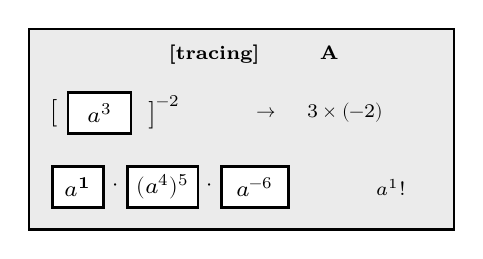
\begin{tikzpicture}[x=1cm, y=1cm, every node/.style={font=\scriptsize, text=black}]
      \draw[black, line width=0.8pt, fill=panelgray] (0,0) rectangle (5.40, 2.55);
      \node[font=\scriptsize] at (2.70, 2.22) {\textbf{ដាន \en{[tracing]} បេសកកម្ម \en{A}}};
      \node[font=\small] at (0.32, 1.48) {$\big[$};
      \draw[black, line width=0.95pt, fill=white] (0.50, 1.22) rectangle (1.30, 1.74);
      \node[font=\footnotesize] at (0.90, 1.48) {$a^3$};
      \node[font=\small] at (1.72, 1.48) {$\big]^{-2}$};
      \node[font=\scriptsize] at (3.70, 1.48) {$\to$ គុណ $3 \times (-2)$};
      \draw[black, line width=0.95pt, fill=white] (0.30, 0.28) rectangle (0.95, 0.80);
      \node[font=\footnotesize] at (0.62, 0.54) {$a^{\mathbf{1}}$};
      \node[font=\footnotesize] at (1.10, 0.54) {$\cdot$};
      \draw[black, line width=0.95pt, fill=white] (1.25, 0.28) rectangle (2.15, 0.80);
      \node[font=\footnotesize] at (1.70, 0.54) {$(a^4)^5$};
      \node[font=\footnotesize] at (2.30, 0.54) {$\cdot$};
      \draw[black, line width=0.95pt, fill=white] (2.45, 0.28) rectangle (3.30, 0.80);
      \node[font=\footnotesize] at (2.87, 0.54) {$a^{-6}$};
      \node[font=\scriptsize] at (4.35, 0.54) {បង្ហាញ $a^1$!};
    \end{tikzpicture}\par\vspace{7pt}}
    \chkbox\ ព័ទ្ធ $[a^3]^{-2}$ និងបង្ហាញ $a = a^{\expbox}$។\par\vspace{6pt}
    \chkbox\ \textbf{\en{Pause-Ask!}} ហេតុអ្វី $(a^3)^{-2}$ មិនមែន $a^{3+(-2)}$? ហើយ $a$ គ្មាននិទស្សន្តលើក្បាលស្មើ $a^?$
    &
    \fontsize{8.0pt}{12.0pt}\selectfont
    \textbf{ក.} $(a^3)^{-2} = a^{3\cdot(\expbox)}$ \hfill (\cblank)\par\vspace{7pt}
    \hspace*{1.2em} $= a^{\expbox} = \dfrac{1}{a^{\expbox}}$ ($a\neq 0$) \hfill (\cblank)\par\vspace{12pt}
    \textbf{ខ.} $a \cdot (a^4)^5 \cdot a^{-6}$\par\vspace{7pt}
    \hspace*{1.2em} $= a^{\expbox} \cdot a^{\expbox} \cdot a^{-6}$ \hfill (\cblank, \cblank)\par\vspace{7pt}
    \hspace*{1.2em} $= a^{\expbox[1.10cm]} = a^{\expbox}$ ($a\neq 0$) \hfill (\cblank)\par\vspace{6pt}
    \textit{ផ្ទៀង៖} $\underline{\hspace{4.6cm}}$
    &
    \fontsize{7.7pt}{11.2pt}\selectfont
    \chkbox\ \textbf{\en{Pause-Review!}} ពិនិត្យ៖\par\vspace{5pt}
    ១) លក្ខខណ្ឌ $a \neq 0$ ត្រូវបានបញ្ជាក់ព្រោះមាននិទស្សន្តដក (\cnum{5}) ឬទេ?\par\vspace{5pt}
    ២) $a^{-6} = \dfrac{1}{a^6}$ ពិត (មិនមែន $-\dfrac{1}{a^6}$ ឬ $-a^6$!)។\par\vspace{5pt}
    ៣) លេខហេតុផល \cnum{1}, \cnum{4}, \cnum{5} ត្រូវគ្រប់ជំហាន!\par\vspace{10pt}
    \begin{tcolorbox}[enhanced, sharp corners, colback=panelgray, colframe=black, boxrule=0.7pt, boxsep=1pt, top=5pt, bottom=5pt, left=4.5pt, right=4.5pt]
      \fontsize{7.4pt}{10.5pt}\selectfont
      \chkbox\ \textbf{ហត្ថលេខាក្រុម \en{A}៖} $\underline{\hspace{1.8cm}}$\\[3pt]
      \textbf{លេខហេតុផល៖} \underline{\hspace{2.1cm}}
    \end{tcolorbox}
    \\ \hline
  \end{tabular}\par}
  \vspace{9pt}
  {\centering\fontsize{7.3pt}{10.2pt}\selectfont \textbf{ធនាគារ \cnum{1}--\cnum{5}៖} \cnum{1} $(a^m)^n=a^{mn}$ \en{|} \cnum{2} $(ab)^n=a^nb^n$ \en{|} \cnum{3} $a^nb^n=(ab)^n$ \en{|} \cnum{4} $a^ma^n=a^{m+n}, a=a^1$ \en{|} \cnum{5} $a^{-n}=\frac{1}{a^n}, -c(ab)^n\neq(-cab)^n$\par}
\end{tcolorbox}

\vspace{22pt}
\noindent\scissors\ \dotfill\ \textbf{កាត់តាមស្នាមចុចចែកជា ២ បេសកកម្ម (\en{Cut Along Dashed Line})} \dotfill\ \scissors
\vspace{22pt}

% --- Mission B: ប្រតិបត្តិ ៤.២ (ទំ.១៨ ដើម) ---
\begin{tcolorbox}[
  enhanced, sharp corners, colback=white, colframe=white,
  borderline={1.0pt}{0pt}{black, dashed},
  boxsep=1pt, top=12pt, bottom=12pt, left=5.5pt, right=5.5pt
]
  \begin{tcolorbox}[
    enhanced, sharp corners, colback=headgray, colframe=black,
    boxrule=0.85pt, boxsep=1pt, top=4.5pt, bottom=4.5pt, left=5.5pt, right=5.5pt, after skip=8pt
  ]
    \fontsize{8.3pt}{11.5pt}\selectfont
    \textbf{\scissors\ បេសកកម្ម \en{B} \en{--} ប្រតិបត្តិ ៤.២ (ទំ.១៨ ដើម)៖} គណនា ($a, b \neq 0$)៖ \textbf{ក.} $-2(a^{-3}\cdot b^5)^2$ \qquad \textbf{ខ.} $a \cdot (a^4) \cdot a^{-6}$ \hfill ក្រុម៖ $\underline{\hspace{2.3cm}}$
  \end{tcolorbox}

  \renewcommand{\arraystretch}{1.42}
  {\centering\setlength{\tabcolsep}{4.5pt}%
  \begin{tabular}{|L{5.65cm}|L{6.45cm}|L{5.25cm}|}
    \hline
    \cellcolor{panelgray}\centering\arraybackslash\fontsize{7.8pt}{10.8pt}\selectfont\textbf{តួនាទី ១៖ អ្នកគូសសញ្ញា \en{B\&W [tracing]}}\newline {\fontsize{7.1pt}{9.8pt}\selectfont \en{\& Pause-Ask!} (ជញ្ជាំង $-2$ \& សង្កេត $(a^4)$)} &
    \cellcolor{panelgray}\centering\arraybackslash\fontsize{7.8pt}{10.8pt}\selectfont\textbf{តួនាទី ២៖ អ្នកភ្ជាប់ហេតុផល \cnum{1}--\cnum{5} \& គណនា}\newline {\fontsize{7.1pt}{9.8pt}\selectfont អនុវត្តជំហានគណនា និងចុះលេខ \cnum{1}--\cnum{5}} &
    \cellcolor{panelgray}\centering\arraybackslash\fontsize{7.8pt}{10.8pt}\selectfont\textbf{តួនាទី ៣៖ អ្នកត្រួតពិនិត្យសញ្ញាដក/លក្ខខណ្ឌ}\newline {\fontsize{7.1pt}{9.8pt}\selectfont \en{\& Pause-Review!} (ធៀបទំ.១៨ vs ១៧)} \\ \hline

    \fontsize{7.7pt}{11.2pt}\selectfont
    {\centering
    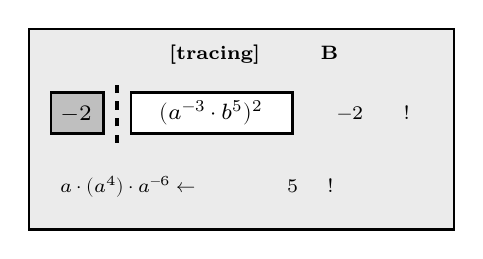
\begin{tikzpicture}[x=1cm, y=1cm, every node/.style={font=\scriptsize, text=black}]
      \draw[black, line width=0.8pt, fill=panelgray] (0,0) rectangle (5.40, 2.55);
      \node[font=\scriptsize] at (2.70, 2.22) {\textbf{ដាន \en{[tracing]} បេសកកម្ម \en{B}}};
      \draw[black, line width=0.95pt, fill=midgray] (0.28, 1.22) rectangle (0.95, 1.74);
      \node[font=\footnotesize] at (0.61, 1.48) {$-2$};
      \draw[black, dashed, line width=1.15pt] (1.12, 1.10) -- (1.12, 1.85);
      \draw[black, line width=0.95pt, fill=white] (1.30, 1.22) rectangle (3.35, 1.74);
      \node[font=\footnotesize] at (2.32, 1.48) {$(a^{-3}\cdot b^5)^2$};
      \node[font=\scriptsize] at (4.38, 1.48) {$-2$ នៅក្រៅ!};
      \node[anchor=west, font=\scriptsize] at (0.28, 0.54) {$a\cdot (a^4)\cdot a^{-6} \leftarrow$ \textbf{គ្មាន}និទស្សន្ត $5$ ក្រៅ!};
    \end{tikzpicture}\par\vspace{7pt}}
    \chkbox\ គូសជញ្ជាំងផ្ដាច់ $-2 \parallel (a^{-3}\cdot b^5)^2$។\par\vspace{6pt}
    \chkbox\ \textbf{\en{Pause-Ask!}} ហេតុអ្វី $-2$ មិនលើកស្វ័យគុណ $2$ ទៅជា $+4$? ហើយទំ.១៨ $(a^4)$ ខុសពីទំ.១៧ $(a^4)^5$ ត្រង់ណា?
    &
    \fontsize{8.0pt}{12.0pt}\selectfont
    \textbf{ក.} $-2(a^{-3}\cdot b^5)^2$\par\vspace{7pt}
    \hspace*{1.2em} $= -2 \cdot (a^{-3})^{\expbox} \cdot (b^5)^{\expbox}$ \hfill (\cblank, \cblank)\par\vspace{7pt}
    \hspace*{1.2em} $= -2 \cdot a^{\expbox} \cdot b^{\expbox} = -\dfrac{2b^{\expbox}}{a^{\expbox}}$ \hfill (\cblank, \cblank)\par\vspace{11pt}
    \textbf{ខ.} $a \cdot (a^4) \cdot a^{-6} = a^{\expbox} \cdot a^4 \cdot a^{-6}$\par\vspace{7pt}
    \hspace*{1.2em} $= a^{1+4-6} = a^{\expbox} = \dfrac{1}{a}$ ($a\neq 0$) \hfill (\cblank, \cblank)\par\vspace{6pt}
    \textit{ផ្ទៀង៖} $\underline{\hspace{4.6cm}}$
    &
    \fontsize{7.7pt}{11.2pt}\selectfont
    \chkbox\ \textbf{\en{Pause-Review!}} ពិនិត្យ៖\par\vspace{5pt}
    ១) មេគុណ $-2$ រក្សាទុកដដែល (មិនមែន $(-2)^2=+4$!) និង $a,b\neq 0$។\par\vspace{5pt}
    ២) \textbf{ប្រៀបធៀបសៀវភៅ៖} ទំ.១៧ (ខ) មាន $(a^4)^5 \Rightarrow a^{15}$ រីឯទំ.១៨ (ខ) មាន $(a^4)$ គ្មាន $5 \Rightarrow a^{-1} = \frac{1}{a}$!\par\vspace{9pt}
    \begin{tcolorbox}[enhanced, sharp corners, colback=panelgray, colframe=black, boxrule=0.7pt, boxsep=1pt, top=5pt, bottom=5pt, left=4.5pt, right=4.5pt]
      \fontsize{7.2pt}{10.2pt}\selectfont
      \textbf{បិទបេសកកម្ម \en{E1}៖} បូណាត្រូវទាំងពីរ $(2^3)^4 = 2^{12} = 4,096$ (\cnum{1}) និង $(3b)^2 = 9b^2$ (\cnum{2})!\\[2pt]
      \chkbox\ \textbf{ហត្ថលេខាក្រុម \en{B}៖} $\underline{\hspace{1.8cm}}$
    \end{tcolorbox}
    \\ \hline
  \end{tabular}\par}
  \vspace{9pt}
  {\centering\fontsize{7.3pt}{10.2pt}\selectfont \textbf{ធនាគារ \cnum{1}--\cnum{5}៖} \cnum{1} $(a^m)^n=a^{mn}$ \en{|} \cnum{2} $(ab)^n=a^nb^n$ \en{|} \cnum{3} $a^nb^n=(ab)^n$ \en{|} \cnum{4} $a^ma^n=a^{m+n}, a=a^1$ \en{|} \cnum{5} $a^{-n}=\frac{1}{a^n}, -c(ab)^n\neq(-cab)^n$\par}
\end{tcolorbox}

\clearpage

% ============================================================================
% ទំព័រទី ៤៖ ផ្ទាំងសំអាងមេរៀន ២.៤.១ & ២.៤.២ (ប្រអប់ "ជាទូទៅ" ទំ.១៧ + ធនាគារ ①–⑤ + អន្ទាក់ ៣)
% ============================================================================
\begin{tcolorbox}[
  enhanced, sharp corners, colback=white, colframe=black,
  boxrule=1.5pt, borderline={0.6pt}{2.2pt}{black},
  boxsep=1pt, top=14pt, bottom=14pt, left=7pt, right=7pt
]
  \begin{center}
    {\fontsize{8.5pt}{11.8pt}\selectfont មន្ទីរអប់រំ យុវជន និងកីឡា ខេត្តកំពង់ធំ \en{|} ការិយាល័យអប់រំ យុវជន និងកីឡា ស្រុកកំពង់ស្វាយ \en{|} អនុវិទ្យាល័យព្រះក្រសាំង}\\[4pt]
    {\muol\fontsize{11.4pt}{17.0pt}\selectfont ផ្ទាំងសំអាងមេរៀន ២\enbf{.}៤\enbf{.}១ \enbf{\&} ២\enbf{.}៤\enbf{.}២៖ ស្វ័យគុណនៃស្វ័យគុណ និងផលគុណ \enbf{(}\cnum{1}\enbf{--}\cnum{5}\enbf{)}}\\[4pt]
    {\fontsize{7.9pt}{11.2pt}\selectfont គណិតវិទ្យា ថ្នាក់ទី៨ \en{--} មេរៀនទី២ (ទំ.១៧\en{--}១៨ ដើម) \en{|} គ្រូបង្រៀន៖ ហុក ប៊ុនថែន \en{|} ឆ្នាំមមី អដ្ឋស័ក ព.ស. ២៥៧០ \en{/} ២០២៦}\\[5pt]
    \khmflourish
  \end{center}
  \vspace{12pt}

  % --- ផ្នែកទី ១៖ ប្រអប់ "ជាទូទៅ" ទាំងពីររបស់ MoEYS ទំ.១៧ ---
  \noindent
  \begin{minipage}[t]{8.80cm}
    \begin{tcolorbox}[
      enhanced, sharp corners, colback=white, colframe=black,
      boxrule=0.95pt, boxsep=1pt, equal height group=posterTopEXP,
      top=10pt, bottom=10pt, left=6pt, right=6pt,
      title={\textbf{៤.១ ស្វ័យគុណនៃស្វ័យគុណ (ទំ.១៧)}},
      colbacktitle=headgray, coltitle=black, fonttitle=\fontsize{8.7pt}{12.0pt}\selectfont
    ]
      \raggedright\fontsize{8.3pt}{12.2pt}\selectfont
      \textbf{ជាទូទៅ៖} បើ $a$ ជាចំនួនសនិទាន និង $m, n$ ជាចំនួនគត់រ៉ឺឡាទីបខុសពីសូន្យ គេបាន៖
      \[
        (a^m)^n = (a^n)^m = a^{m\cdot n}
      \]
      \textit{(លក្ខខណ្ឌសុក្រឹត៖ បើ $m < 0$, $n < 0$ ឬស្មើ $0$ ត្រូវ $a \neq 0$ ដើម្បីចៀសវាង $0^{-k}$ ឬ $0^0$ គ្មានន័យ)។}\\[8pt]
      \centering
      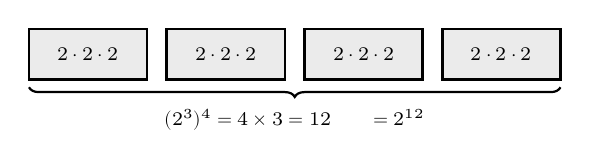
\begin{tikzpicture}[x=1cm, y=1cm, every node/.style={font=\scriptsize, text=black}]
        \foreach \i/\xoff in {1/0, 2/1.75, 3/3.50, 4/5.25}{
          \draw[black, line width=0.95pt, fill=panelgray] (\xoff, 0) rectangle (\xoff+1.50, 0.64);
          \node at (\xoff+0.75, 0.32) {$2\cdot 2\cdot 2$};
        }
        \draw[decorate, decoration={brace, mirror, amplitude=3.5pt}, line width=0.8pt] (0, -0.10) -- (6.75, -0.10)
          node[midway, below=4pt] {$(2^3)^4 = 4 \times 3 = 12$ កត្តា $= 2^{12}$};
      \end{tikzpicture}
    \end{tcolorbox}
  \end{minipage}\hfill
  \begin{minipage}[t]{8.80cm}
    \begin{tcolorbox}[
      enhanced, sharp corners, colback=panelgray, colframe=black,
      boxrule=0.95pt, boxsep=1pt, equal height group=posterTopEXP,
      top=10pt, bottom=10pt, left=6pt, right=6pt,
      title={\textbf{៤.២ ស្វ័យគុណនៃផលគុណ (ទំ.១៧)}},
      colbacktitle=headgray, coltitle=black, fonttitle=\fontsize{8.7pt}{12.0pt}\selectfont
    ]
      \raggedright\fontsize{8.3pt}{12.2pt}\selectfont
      \textbf{ជាទូទៅ៖} បើ $a, b$ ជាចំនួនសនិទាន និង $n$ ជាចំនួនគត់រ៉ឺឡាទីបខុសពីសូន្យ គេបាន៖
      \[
        (a \cdot b)^n = a^n \cdot b^n \quad \text{និងច្រាស} \quad a^n \cdot b^n = (a \cdot b)^n
      \]
      \textit{(លក្ខខណ្ឌសុក្រឹត៖ បើ $n < 0$ ឬស្មើ $0$ ត្រូវ $a \neq 0$ និង $b \neq 0$)។}\\[8pt]
      \centering
      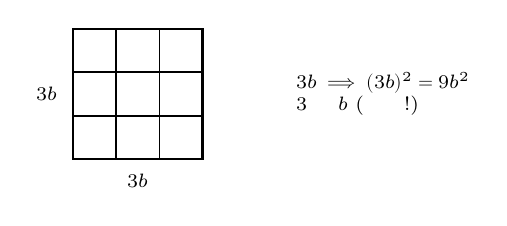
\begin{tikzpicture}[x=1cm, y=1cm, every node/.style={font=\scriptsize, text=black}]
        \draw[black, line width=1.0pt, fill=white] (0, 0) rectangle (1.65, 1.65);
        \draw[black, line width=0.65pt] (0.55, 0)--(0.55, 1.65) (1.10, 0)--(1.10, 1.65);
        \draw[black, line width=0.65pt] (0, 0.55)--(1.65, 0.55) (0, 1.10)--(1.65, 1.10);
        \node[left=2pt, font=\scriptsize] at (0, 0.825) {$3b$};
        \node[below=2pt, font=\scriptsize] at (0.825, 0) {$3b$};
        \node[right=5pt, align=left] at (1.75, 0.825) {ការ៉េជ្រុង $3b \implies (3b)^2 = 9b^2$\\ចែកឱ្យទាំង $3$ និង $b$ (៩ ក្រឡា!)};
      \end{tikzpicture}
    \end{tcolorbox}
  \end{minipage}

  \vspace{13pt}

  % --- ផ្នែកទី ២៖ តារាងធនាគារហេតុផល ①–⑤ (Word-for-Word ១០០% នឹង LS_Plan_EXP412) ---
  \fontsize{8.3pt}{12.2pt}\selectfont
  \renewcommand{\arraystretch}{1.95}
  \begin{tabular}{|C{0.72cm}|L{4.20cm}|L{6.05cm}|C{5.10cm}|}
    \hline
    \cellcolor{headgray}\textbf{លេខ} &
    \cellcolor{headgray}\centering\arraybackslash\textbf{ឈ្មោះហេតុផល (\en{Warrant})} &
    \cellcolor{headgray}\centering\arraybackslash\textbf{រូបមន្ត និងលក្ខខណ្ឌកំណត់} &
    \cellcolor{headgray}\centering\arraybackslash\textbf{ដ្យាក្រាមវង់ក្រចក ស-ខ្មៅ} \\ \hline

    \cnum{1} &
    \textbf{ស្វ័យគុណនៃស្វ័យគុណ (៤.១)} &
    $(a^m)^n = (a^n)^m = a^{m\cdot n}$ \newline \textit{(បើ $m, n < 0$ ត្រូវ $a \neq 0$; គុណនិទស្សន្តនឹងនិទស្សន្ត)} &
    \raisebox{-0.35\height}{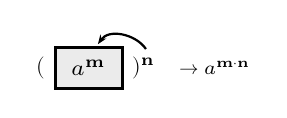
\begin{tikzpicture}[x=1cm, y=1cm, every node/.style={font=\footnotesize, text=black}]
      \node at (-0.18,0.28) {$($};
      \draw[black, line width=0.95pt, fill=panelgray] (0,0.02) rectangle (0.85,0.54);
      \node at (0.42,0.28) {$a^{\mathbf{m}}$};
      \node at (1.12,0.28) {$)^{\mathbf{n}}$};
      \draw[black, line width=0.8pt, -{Stealth[length=1.2mm]}] (1.15,0.52) to[out=125, in=55] (0.54,0.58);
      \node[right=2pt, font=\scriptsize] at (1.38,0.28) {$\to a^{\mathbf{m\cdot n}}$};
    \end{tikzpicture}} \\ \hline

    \cnum{2} &
    \textbf{ស្វ័យគុណនៃផលគុណ — ចែកនិទស្សន្ត (៤.២ ផ្ទាល់)} &
    $(a \cdot b)^n = a^n \cdot b^n$ \newline \textit{(ចែក $n$ ឱ្យគ្រប់កត្តា រួមទាំងមេគុណលេខ; $a,b\neq 0$ បើ $n<0$)} &
    \raisebox{-0.35\height}{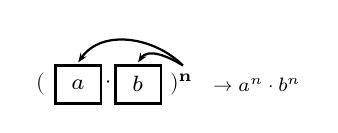
\begin{tikzpicture}[x=1cm, y=1cm, every node/.style={font=\footnotesize, text=black}]
      \node at (-0.18,0.26) {$($};
      \draw[black, line width=0.95pt] (0,0.02) rectangle (0.58,0.50);
      \draw[black, line width=0.95pt] (0.76,0.02) rectangle (1.34,0.50);
      \node at (0.29,0.26) {$a$}; \node at (0.67,0.26) {$\cdot$}; \node at (1.05,0.26) {$b$};
      \node at (1.60,0.26) {$)^{\mathbf{n}}$};
      \draw[black, line width=0.8pt, -{Stealth[length=1.2mm]}] (1.62,0.50) to[out=135, in=55] (0.29,0.54);
      \draw[black, line width=0.8pt, -{Stealth[length=1.2mm]}] (1.62,0.50) to[out=148, in=55] (1.05,0.54);
      \node[right=2pt, font=\scriptsize] at (1.82,0.26) {$\to a^n\cdot b^n$};
    \end{tikzpicture}} \\ \hline

    \cnum{3} &
    \textbf{ស្វ័យគុណនៃផលគុណ — ផ្គុំគោលគុណ (៤.២ ច្រាស)} &
    $a^n \cdot b^n = (a \cdot b)^n$ \newline \textit{(ពេលនិទស្សន្ត $n$ ដូចគ្នា អាចផ្គុំគោល $a\cdot b$ ចូលវង់ក្រចក)} &
    \raisebox{-0.35\height}{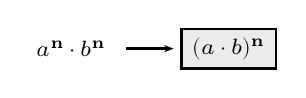
\begin{tikzpicture}[x=1cm, y=1cm, every node/.style={font=\footnotesize, text=black}]
      \node at (0.35,0.28) {$a^{\mathbf{n}} \cdot b^{\mathbf{n}}$};
      \draw[black, line width=0.85pt, -{Stealth[length=1.2mm]}] (1.05,0.28) -- (1.65,0.28);
      \draw[black, line width=0.95pt, fill=panelgray] (1.75,0.03) rectangle (2.95,0.53);
      \node at (2.35,0.28) {$(a\cdot b)^{\mathbf{n}}$};
    \end{tikzpicture}} \\ \hline

    \cnum{4} &
    \textbf{ផលគុណគោលដូចគ្នា (២.២)} &
    $a^m \cdot a^n = a^{m+n}$ និង $a = a^1$ \newline \textit{(គោលដូចគ្នាគុណគ្នា $\to$ បូកនិទស្សន្ត; កុំភ្លេច $a = a^1$)} &
    \raisebox{-0.35\height}{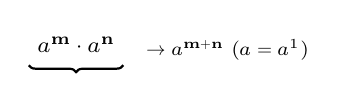
\begin{tikzpicture}[x=1cm, y=1cm, every node/.style={font=\footnotesize, text=black}]
      \node at (0.65,0.34) {$a^{\mathbf{m}} \cdot a^{\mathbf{n}}$};
      \draw[decorate, decoration={brace, mirror, amplitude=2.5pt}, line width=0.8pt] (0.05,0.08) -- (1.25,0.08);
      \node[right=2pt, font=\scriptsize] at (1.35,0.28) {$\to a^{\mathbf{m+n}}$ ($a=a^1$)};
    \end{tikzpicture}} \\ \hline

    \cnum{5} &
    \textbf{និទស្សន្តអវិជ្ជមាន/សូន្យ \& វិសាលភាពសញ្ញាដក} &
    $a^{-n} = \dfrac{1}{a^n},\;\; a^0 = 1\; (a\neq 0)$ \newline និង $-c(ab)^n \neq (-cab)^n$ \textit{(មេគុណក្រៅវង់ក្រចក!)} &
    \raisebox{-0.35\height}{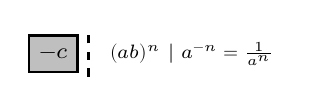
\begin{tikzpicture}[x=1cm, y=1cm, every node/.style={font=\footnotesize, text=black}]
      \draw[black, line width=0.9pt, fill=midgray] (0,0.04) rectangle (0.62,0.50);
      \node at (0.31,0.27) {$-c$};
      \draw[black, dashed, line width=1.15pt] (0.76,-0.02) -- (0.76,0.58);
      \node[right=2pt, font=\scriptsize] at (0.84,0.27) {$(ab)^n$ \en{|} $a^{-n}=\frac{1}{a^n}$};
    \end{tikzpicture}} \\ \hline
  \end{tabular}

  \vspace{13pt}

  % --- ផ្នែកទី ៣៖ ប្រអប់ព្រមាន "ប្រយ័ត្នអន្ទាក់ទាំង ៣" ---
  \begin{tcolorbox}[
    enhanced, sharp corners, colback=white, colframe=black,
    boxrule=1.15pt, boxsep=1pt, top=10pt, bottom=10pt, left=7pt, right=7pt,
    title={\ding{55}\ \textbf{ប្រយ័ត្នអន្ទាក់ទាំង ៣ (កំហុសញឹកញាប់បំផុតក្នុងថ្នាក់ទី៨)}},
    colbacktitle=midgray, coltitle=black, fonttitle=\fontsize{9.2pt}{12.5pt}\selectfont
  ]
    \raggedright\fontsize{8.5pt}{13.0pt}\selectfont
    \textbf{១. អន្ទាក់បូកនិទស្សន្តឆ្លងវង់ក្រចក៖} $(a^m)^n \neq a^{m+n}$ \quad (ឧ. $(2^3)^4 = 2^{3\times 4} = 2^{12}$ មិនមែន $2^{3+4} = 2^7$ ទេ! \cnum{1} vs \cnum{4})\\[7pt]
    \textbf{២. អន្ទាក់លីនេអ៊ែរ (\en{Freshman's Dream})៖} $(a + b)^n \neq a^n + b^n$ \quad (ឧ. $(2+3)^2 = 25 \neq 2^2+3^2 = 13$; ចែកបានតែ\textbf{ផលគុណ} \cnum{2}!)\\[7pt]
    \textbf{៣. អន្ទាក់មេគុណ \& សញ្ញាដកក្រៅវង់ក្រចក៖} $-2(ab)^2 = -2a^2b^2 \neq (-2ab)^2 = 4a^2b^2$ និង $(3xy^2)^3 = 27x^3y^6 \neq 3x^3y^6$ (\cnum{2}, \cnum{5})!
  \end{tcolorbox}

  \vspace{12pt}
  \begin{tcolorbox}[
    enhanced, sharp corners, colback=panelgray, colframe=black,
    boxrule=0.75pt, boxsep=1pt, top=7pt, bottom=7pt, left=6pt, right=6pt
  ]
    \centering\fontsize{8.2pt}{11.8pt}\selectfont
    \textbf{គោលការណ៍ប្រើផ្ទាំងសំអាងក្នុងថ្នាក់ (\en{E3--E5})៖} រាល់ជំហានដោះស្រាយក្នុង \textbf{លំហាត់គំរូ (ទំ.១៧--១៨)}, \textbf{ប្រតិបត្តិ} និង \textbf{កិច្ចការផ្ទះ (ទំ.២៥--២៦)} ត្រូវចុះលេខហេតុផល \cnum{1}--\cnum{5} ភ្ជាប់ជានិច្ច!
  \end{tcolorbox}
\end{tcolorbox}

\clearpage

% ============================================================================
% ទំព័រទី ៥៖ កាតវិនិច្ឆ័យរហ័ស E5 (កាត A / B / C / D) + ចម្លើយគ្រូ & ការកែតម្រូវ
% ============================================================================
\pagebanner{សម្ភារៈទី ៥៖ កាតវិនិច្ឆ័យរហ័ស «កាត \enbf{A--D}» \enbf{\&} គន្លឹះកែតម្រូវគ្រូ \enbf{E5}}{ទំព័រ ៥/៦ \en{-- E5 Evaluate}}

{\fontsize{8.5pt}{12.0pt}\selectfont
\textbf{សំណួរចម្បង (\en{E5} លើកកាតបង្ហាញ ឬបង្ហាញចង្អុលម្រាម \en{A--D})៖} «តើសមភាពមួយណា\textbf{ត្រឹមត្រូវ (\ding{51})} ចំពោះគ្រប់ $x, y \neq 0$?»}

\vspace{11pt}

% --- ជួរទី ១៖ កាត A & កាត B ---
\noindent
\begin{tcolorbox}[
  enhanced, sharp corners, colback=white, colframe=white,
  borderline={1.0pt}{0pt}{black, dashed},
  width=9.25cm, equal height group=expfoilrow1, nobeforeafter,
  boxsep=1pt, top=11pt, bottom=11pt, left=6pt, right=6pt
]
  \noindent\colorbox{black}{\textcolor{white}{\Large\textbf{\en{ A }}}}\hspace{0.22cm}{\fontsize{9.2pt}{12.5pt}\selectfont\textbf{កាត \en{A} ៖ ស្វ័យគុណនៃស្វ័យគុណ}}\par\vspace{14pt}
  \begin{center}
    {\fontsize{18.5pt}{22pt}\selectfont $\displaystyle (x^4)^3 \;=\; x^7$}
  \end{center}
  \vspace{12pt}
  \begin{center}
  
\begin{tikzpicture}[x=1cm, y=1cm, every node/.style={font=\footnotesize, text=black}]
    \draw[black, line width=0.9pt, fill=panelgray] (0,0) rectangle (7.7, 0.86);
    \node at (3.85, 0.43) {ផ្ទៀង៖ តើ $4$ និង $3$ ត្រូវ \textbf{បូក} ឬ \textbf{គុណ}? (\cnum{1} vs \cnum{4})};
  \end{tikzpicture}
  \end{center}
  \vspace{7pt}
  {\centering\fontsize{8.0pt}{11pt}\selectfont ហេតុផល / លេខ \cnum{1}--\cnum{5}៖ $\underline{\hspace{4.8cm}}$\par}
  \vfill
  \begin{tcolorbox}[enhanced, sharp corners, colback=panelgray, colframe=black, boxrule=0.8pt, boxsep=1pt, top=5pt, bottom=5pt, left=4pt, right=4pt]
    \centering\fontsize{8.8pt}{11.8pt}\selectfont
    \textbf{វិនិច្ឆ័យ៖} \quad \chkbox~ពិត (\ding{51}) \qquad \chkbox~ខុស (\ding{55})
  \end{tcolorbox}
\end{tcolorbox}%
\hfill
\begin{tcolorbox}[
  enhanced, sharp corners, colback=white, colframe=white,
  borderline={1.0pt}{0pt}{black, dashed},
  width=9.25cm, equal height group=expfoilrow1, nobeforeafter,
  boxsep=1pt, top=11pt, bottom=11pt, left=6pt, right=6pt
]
  \noindent\colorbox{black}{\textcolor{white}{\Large\textbf{\en{ B }}}}\hspace{0.22cm}{\fontsize{9.2pt}{12.5pt}\selectfont\textbf{កាត \en{B} ៖ ស្វ័យគុណនៃផលគុណ (មានមេគុណអវិជ្ជមាន)}}\par\vspace{14pt}
  \begin{center}
    {\fontsize{18.5pt}{22pt}\selectfont $\displaystyle (-2x^3y)^2 \;=\; -2x^6y^2$}
  \end{center}
  \vspace{12pt}
  \begin{center}
  
\begin{tikzpicture}[x=1cm, y=1cm, every node/.style={font=\footnotesize, text=black}]
    \draw[black, line width=0.9pt, fill=panelgray] (0,0) rectangle (7.7, 0.86);
    \node at (3.85, 0.43) {ផ្ទៀង៖ តើ $-2$ នៅ\textbf{ក្នុង} ឬ\textbf{ក្រៅ}វង់ក្រចក? (\cnum{2}, \cnum{5})};
  \end{tikzpicture}
  \end{center}
  \vspace{7pt}
  {\centering\fontsize{8.0pt}{11pt}\selectfont ហេតុផល / លេខ \cnum{1}--\cnum{5}៖ $\underline{\hspace{4.8cm}}$\par}
  \vfill
  \begin{tcolorbox}[enhanced, sharp corners, colback=panelgray, colframe=black, boxrule=0.8pt, boxsep=1pt, top=5pt, bottom=5pt, left=4pt, right=4pt]
    \centering\fontsize{8.8pt}{11.8pt}\selectfont
    \textbf{វិនិច្ឆ័យ៖} \quad \chkbox~ពិត (\ding{51}) \qquad \chkbox~ខុស (\ding{55})
  \end{tcolorbox}
\end{tcolorbox}

\vspace{13pt}

% --- ជួរទី ២៖ កាត C & កាត D ---
\noindent
\begin{tcolorbox}[
  enhanced, sharp corners, colback=white, colframe=white,
  borderline={1.0pt}{0pt}{black, dashed},
  width=9.25cm, equal height group=expfoilrow2, nobeforeafter,
  boxsep=1pt, top=11pt, bottom=11pt, left=6pt, right=6pt
]
  \noindent\colorbox{black}{\textcolor{white}{\Large\textbf{\en{ C }}}}\hspace{0.22cm}{\fontsize{9.2pt}{12.5pt}\selectfont\textbf{កាត \en{C} ៖ ស្វ័យគុណនៃផលគុណ (៣ កត្តា)}}\par\vspace{14pt}
  \begin{center}
    {\fontsize{18.5pt}{22pt}\selectfont $\displaystyle (-2x^3y)^2 \;=\; 4x^6y^2$}
  \end{center}
  \vspace{12pt}
  \begin{center}
  
\begin{tikzpicture}[x=1cm, y=1cm, every node/.style={font=\footnotesize, text=black}]
    \draw[black, line width=0.9pt, fill=panelgray] (0,0) rectangle (7.7, 0.86);
    \node at (3.85, 0.43) {ផ្ទៀង៖ $\big([-2]\cdot[x^3]\cdot[y^1]\big)^2$ គ្រប់ ៣ កត្តា! (\cnum{1}, \cnum{2})};
  \end{tikzpicture}
  \end{center}
  \vspace{7pt}
  {\centering\fontsize{8.0pt}{11pt}\selectfont ហេតុផល / លេខ \cnum{1}--\cnum{5}៖ $\underline{\hspace{4.8cm}}$\par}
  \vfill
  \begin{tcolorbox}[enhanced, sharp corners, colback=panelgray, colframe=black, boxrule=0.8pt, boxsep=1pt, top=5pt, bottom=5pt, left=4pt, right=4pt]
    \centering\fontsize{8.8pt}{11.8pt}\selectfont
    \textbf{វិនិច្ឆ័យ៖} \quad \chkbox~ពិត (\ding{51}) \qquad \chkbox~ខុស (\ding{55})
  \end{tcolorbox}
\end{tcolorbox}%
\hfill
\begin{tcolorbox}[
  enhanced, sharp corners, colback=white, colframe=white,
  borderline={1.0pt}{0pt}{black, dashed},
  width=9.25cm, equal height group=expfoilrow2, nobeforeafter,
  boxsep=1pt, top=11pt, bottom=11pt, left=6pt, right=6pt
]
  \noindent\colorbox{black}{\textcolor{white}{\Large\textbf{\en{ D }}}}\hspace{0.22cm}{\fontsize{9.2pt}{12.5pt}\selectfont\textbf{កាត \en{D} ៖ កន្សោមផលបូកលើកស្វ័យគុណ}}\par\vspace{14pt}
  \begin{center}
    {\fontsize{18.5pt}{22pt}\selectfont $\displaystyle (x + y)^3 \;=\; x^3 + y^3$}
  \end{center}
  \vspace{12pt}
  \begin{center}
  
\begin{tikzpicture}[x=1cm, y=1cm, every node/.style={font=\footnotesize, text=black}]
    \draw[black, line width=0.9pt, fill=panelgray] (0,0) rectangle (7.7, 0.86);
    \node at (3.85, 0.43) {ផ្ទៀង៖ សាកជំនួស $x=2,\; y=3$! (\cnum{2} អនុវត្តតែគុណ)};
  \end{tikzpicture}
  \end{center}
  \vspace{7pt}
  {\centering\fontsize{8.0pt}{11pt}\selectfont ហេតុផល / លេខ \cnum{1}--\cnum{5}៖ $\underline{\hspace{4.8cm}}$\par}
  \vfill
  \begin{tcolorbox}[enhanced, sharp corners, colback=panelgray, colframe=black, boxrule=0.8pt, boxsep=1pt, top=5pt, bottom=5pt, left=4pt, right=4pt]
    \centering\fontsize{8.8pt}{11.8pt}\selectfont
    \textbf{វិនិច្ឆ័យ៖} \quad \chkbox~ពិត (\ding{51}) \qquad \chkbox~ខុស (\ding{55})
  \end{tcolorbox}
\end{tcolorbox}

\vspace{14pt}

% --- ផ្នែកកាត់ទុកសម្រាប់គ្រូ (Teacher Answer & Diagnostic Remediation Key) ---
\noindent\scissors\ \dotfill\ \textbf{កាត់ទុកសម្រាប់គ្រូ (\en{Teacher Answer \& Diagnostic Remediation Key})} \dotfill\ \scissors

\vspace{10pt}
\begin{tcolorbox}[
  enhanced, sharp corners, colback=panelgray, colframe=black,
  boxrule=0.95pt, boxsep=1pt, top=7pt, bottom=7pt, left=5pt, right=5pt
]
  \fontsize{8.0pt}{11.6pt}\selectfont
  \renewcommand{\arraystretch}{1.35}
  \begin{tabular}{|L{4.20cm}|L{4.35cm}|L{4.25cm}|L{4.35cm}|}
    \hline
    \cellcolor{headgray}\textbf{កាត \en{A} ៖ ខុស (\ding{55})} &
    \cellcolor{headgray}\textbf{កាត \en{B} ៖ ខុស (\ding{55})} &
    \cellcolor{headgray}\textbf{កាត \en{C} ៖ ត្រឹមត្រូវ (\ding{51})} &
    \cellcolor{headgray}\textbf{កាត \en{D} ៖ ខុស (\ding{55})} \\ \hline
    \textbf{អន្ទាក់បូកនិទស្សន្ត!} សិស្សច្រឡំ $(x^4)^3$ ជាមួយ $x^4\cdot x^3$! \newline \textit{សួរភ្លាម៖} «មាន $x^4$ ប៉ុន្មានក្រុម? បើមាន $3$ ក្រុមស្មើ $x^{4\times 3}=x^{12}$ (\cnum{1})!» &
    \textbf{ភ្លេចមេគុណក្នុងវង់ក្រចក!} $-2$ នៅ\textbf{ក្នុង}វង់ក្រចកត្រូវលើកការ៉េ $(-2)^2=+4$! \newline \textit{សួរភ្លាម៖} «វង់ក្រចកព័ទ្ធ $-2$ ឬអត់? បើនៅក្រៅទើបនៅ $-2$ (\cnum{2}, \cnum{5})!» &
    \textbf{ពិត ១០០\%!} ទាំង $3$ កត្តាក្នុងវង់ក្រចកគឺ $(-2)^2=4$, $(x^3)^2=x^6$, $(y^1)^2=y^2$! \newline \textit{បញ្ជាក់៖} ផ្ទៀងដោយ \cnum{2} និង \cnum{1} ($x,y\neq 0$)។ &
    \textbf{អន្ទាក់លីនេអ៊ែរ!} \en{Freshman's Dream} ចែកលើផលបូក! \newline \textit{សួរភ្លាម៖} «សាក $(2+3)^3=125$ តែ $2^3+3^3=8+27=35$ — ខុសគ្នាឆ្ងាយ!» \\ \hline
  \end{tabular}
\end{tcolorbox}

\vspace{10pt}
\begin{tcolorbox}[
  enhanced, sharp corners, colback=white, colframe=black,
  boxrule=0.95pt, boxsep=1pt, top=8pt, bottom=8pt, left=7pt, right=7pt
]
  \raggedright\fontsize{8.2pt}{12.4pt}\selectfont
  \textbf{សំបុត្រចេញរហ័ស ៦០--៩០ វិនាទី (\en{Quick Individual Exit Check})៖}\quad ឈ្មោះ៖ $\underline{\hspace{4.0cm}}$ \quad ថ្នាក់៖ $\underline{\hspace{1.4cm}}$\\[6pt]
  \textbf{១)} គណនា $(m^2)^5 = \underline{\hspace{1.3cm}}$ \qquad \textbf{២)} សម្រួល $(-3ab^2)^2 = \underline{\hspace{1.6cm}}$ \qquad \textbf{៣)} តើ $-2(x^3)^2 = 4x^6$ ពិតឬទេ? \chkbox~ពិត \chkbox~ទេ\\[6pt]
  \textbf{៤)} ហេតុអ្វី $(x+2)^2 \neq x^2 + 4$? ចូរពន្យល់ខ្លី (លេខ \cnum{2} vs \en{Freshman's Dream})៖ $\underline{\hspace{7.6cm}}$\\[6pt]
  \hspace*{1.4em} $\underline{\hspace{17.4cm}}$\\[5pt]
  \textit{\fontsize{7.6pt}{10.8pt}\selectfont (ចម្លើយគ្រូ៖ ១. $m^{10}$; \quad ២. $9a^2b^4$; \quad ៣. ទេ $-2x^6$; \quad ៤. ស្វ័យគុណចែកចាយតែលើផលគុណ មិនចែកលើផលបូកទេ — $(x+2)^2 = x^2+4x+4$!)}
\end{tcolorbox}

\clearpage

% ============================================================================
% ទំព័រទី ៦៖ ប័ណ្ណកិច្ចការផ្ទះ ជំហានទី ៥ — ២ ប័ណ្ណដូចគ្នាក្នុង ១ ទំព័រ A4 (ត្រូវគ្នា ១០០% នឹង LS_Plan)
% ============================================================================
\pagebanner{សម្ភារៈទី ៦៖ ប័ណ្ណកិច្ចការផ្ទះ ជំហានទី ៥ \enbf{--} ២ ប័ណ្ណដូចគ្នាក្នុង ១ ទំព័រ \enbf{A4}}{ទំព័រ ៦/៦ \en{--} ជំហានទី ៥ (កាត់ ២ ប័ណ្ណ \scissors)}

\newcommand{\hwslipTwoEXP}[1]{%
\begin{tcolorbox}[
  enhanced, sharp corners, colback=white, colframe=white,
  borderline={1.0pt}{0pt}{black, dashed},
  boxsep=1pt, top=8pt, bottom=8pt, left=7pt, right=7pt
]
  \begin{tcolorbox}[
    enhanced, sharp corners, colback=headgray, colframe=black,
    boxrule=0.85pt, boxsep=1pt, top=4pt, bottom=4pt, left=6pt, right=6pt, after skip=8pt
  ]
    \fontsize{8.5pt}{11.8pt}\selectfont
    \textbf{\scissors\ កិច្ចការផ្ទះ (#1) \en{|} មេរៀនទី២ (២.៤.១--២.៤.២) ស្វ័យគុណ} \hfill ថ្ងៃទី\makebox[12mm]{\dotfill}\ ខែ\makebox[16mm]{\dotfill}\ ២៥៧០ \en{/} ២០២៦\\[3pt]
    ឈ្មោះសិស្ស៖ $\underline{\hspace{5.8cm}}$ \hspace{0.5cm} ថ្នាក់៖ $\underline{\hspace{1.8cm}}$ \hspace{0.5cm} លេខរៀង៖ $\underline{\hspace{1.4cm}}$
  \end{tcolorbox}

  \fontsize{8.6pt}{13.0pt}\selectfont
  \textbf{ផ្នែក ក (ទំ.២៥ \en{\#2}ក, ច្រាស ៤.២, និងត្រៀម \en{\#7}ង)៖}\\[5pt]
  \hspace*{0.8em}\textbf{១)} គណនា $(4^3)(2^2)$ ដោយប្ដូរ $4 = 2^2$ និងគណនា $25^3 \cdot 4^3$ ដោយប្រើលក្ខណៈច្រាស \cnum{3} ។\\[5pt]
  \hspace*{1.8em} $\bullet$ $(4^3)(2^2) = \underline{\hspace{13.5cm}}$\\[7pt]
  \hspace*{1.8em} $\bullet$ $25^3 \cdot 4^3 = \underline{\hspace{13.7cm}}$\\[8pt]
  \hspace*{0.8em}\textbf{២)} សម្រួលកន្សោម $(-2a^2x^2)^2(-4a^3x)^3$ ។\\[5pt]
  \hspace*{1.8em} $\bullet$ $(-2a^2x^2)^2(-4a^3x)^3 = \underline{\hspace{11.7cm}}$\\[7pt]
  \hspace*{1.8em} \phantom{$\bullet$ $(-2a^2x^2)^2(-4a^3x)^3$ }$= \underline{\hspace{11.7cm}}$

  \vspace{7pt}\hrule height 0.5pt\vspace{7pt}

  \fontsize{8.6pt}{13.0pt}\selectfont
  \textbf{ផ្នែក ខ (ទំ.២៦ \en{\#8}ក,ខ,គ)៖}\\[5pt]
  \hspace*{0.8em}\textbf{១)} សរសេរ $x^{12}$ ជាស្វ័យគុណនៃ $x^2$ និង $y^{15}$ ជាស្វ័យគុណនៃ $y^3$ ។\\[5pt]
  \hspace*{1.8em} $\bullet$ $x^{12} = (\,x^2\,)^{\expbox[0.65cm]}$ \hspace*{2.4cm} $\bullet$ $y^{15} = (\,y^3\,)^{\expbox[0.65cm]}$\\[7pt]
  \hspace*{0.8em}\textbf{២)} សរសេរ $2^{18}$ និង $(2^5)^6$ ជាស្វ័យគុណនៃ $8$ ។\\[5pt]
  \hspace*{1.8em} $\bullet$ $2^{18} = (2^{\expbox})^{\expbox} = 8^{\expbox[0.52cm]}$ \hspace*{1.5cm} $\bullet$ $(2^5)^6 = 2^{\expbox[0.52cm]} = (2^{\expbox})^{\expbox[0.52cm]} = 8^{\expbox[0.52cm]}$

  \vspace{8pt}
  \begin{tcolorbox}[
    enhanced, sharp corners, colback=panelgray, colframe=black,
    boxrule=0.75pt, boxsep=1pt, top=4.5pt, bottom=4.5pt, left=6pt, right=6pt
  ]
    \fontsize{7.9pt}{11.2pt}\selectfont
    \textbf{ផ្ទៀងខ្លួនឯង (\cnum{1}--\cnum{5})៖}
    \chkbox~ចុះលេខហេតុផល \cnum{1}--\cnum{5} \en{|}
    \chkbox~លើកស្វ័យគុណទាំងមេគុណ $(-2)^2, (-4)^3$ \en{|}
    \chkbox~ប្ដូរគោល $8 = 2^3$! \hfill ហត្ថលេខា៖ $\underline{\hspace{2.3cm}}$
  \end{tcolorbox}
\end{tcolorbox}%
}

\vspace{7pt}
\hwslipTwoEXP{ប័ណ្ណទី ១}

\vspace{16pt}
\noindent\scissors\ \dotfill\ \textbf{កាត់តាមស្នាមចុចចែកជា ២ ប័ណ្ណ (\en{Cut Along Dashed Line})} \dotfill\ \scissors
\vspace{16pt}

\hwslipTwoEXP{ប័ណ្ណទី ២}

\end{document}
